% Created by tikzDevice version 0.10.1 on 2016-06-20 06:54:16
% !TEX encoding = UTF-8 Unicode
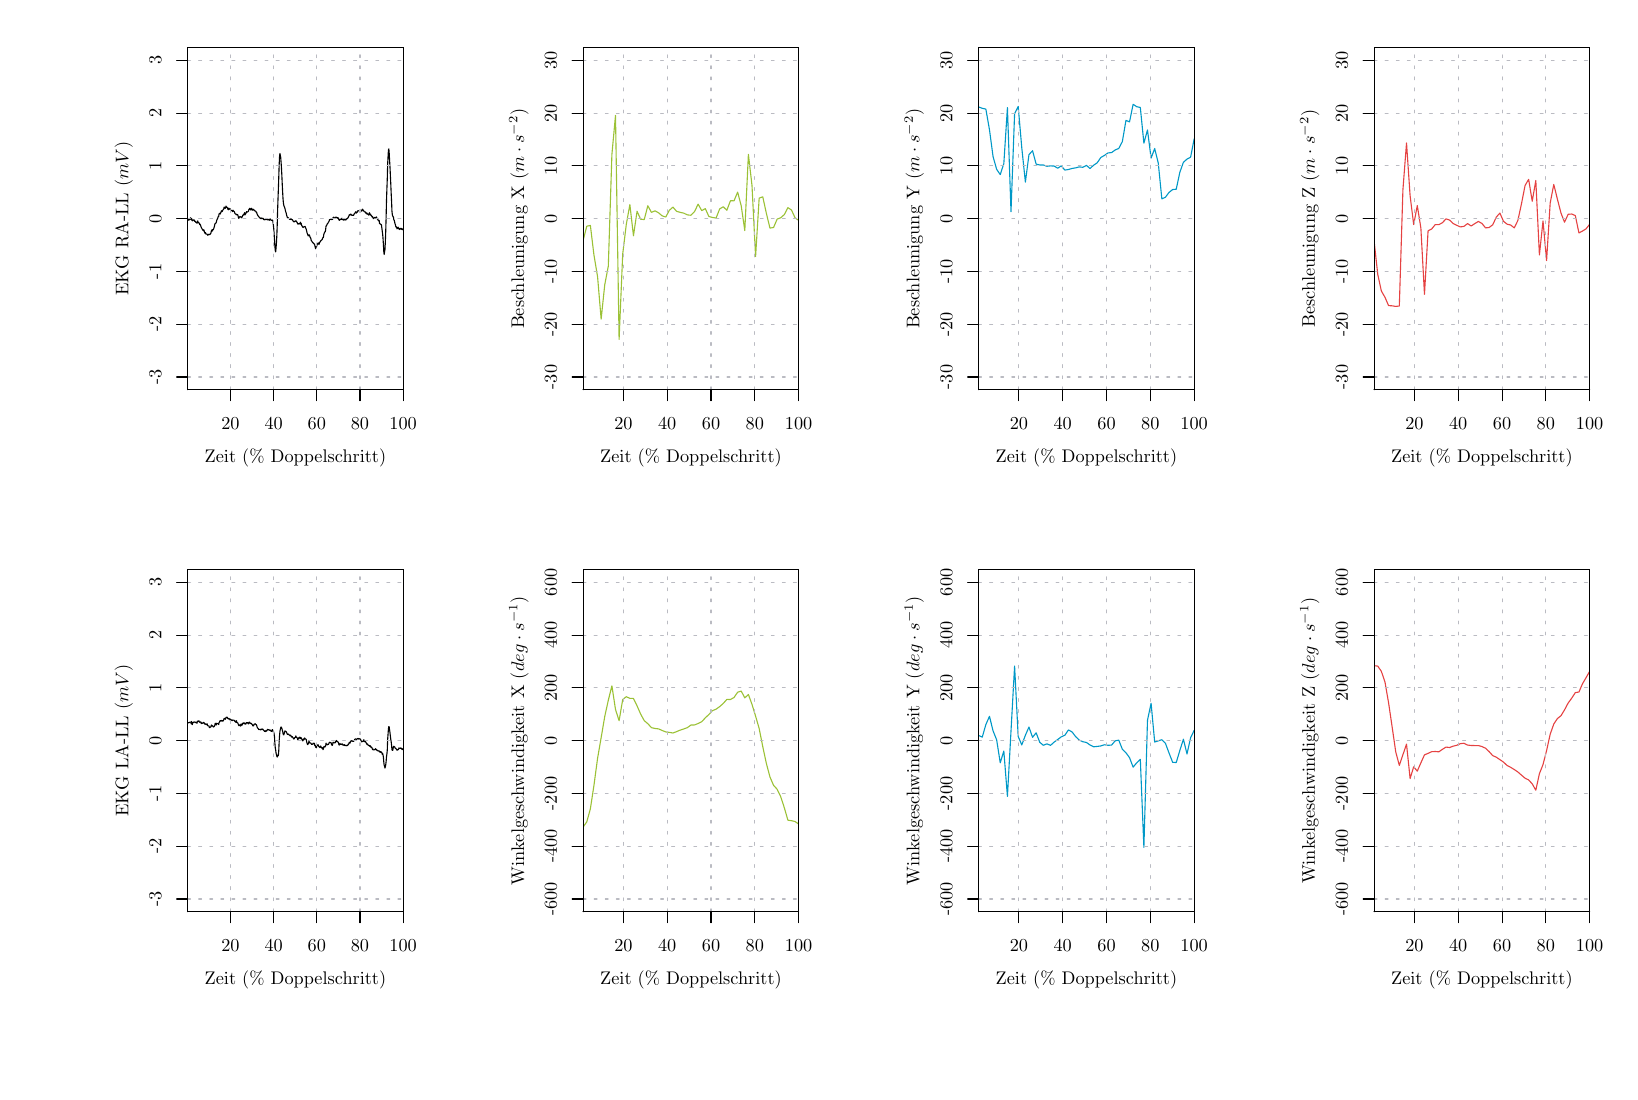
\begin{tikzpicture}[x=1pt,y=1pt]
\definecolor{fillColor}{RGB}{255,255,255}
\path[use as bounding box,fill=fillColor,fill opacity=0.00] (0,0) rectangle (571.66,377.25);
\begin{scope}
\path[clip] ( 57.82,246.44) rectangle (135.69,370.02);
\definecolor{drawColor}{RGB}{0,0,0}

\path[draw=drawColor,line width= 0.4pt,line join=round,line cap=round] ( 57.82,308.23) --
	( 57.96,308.00) --
	( 58.10,308.00) --
	( 58.24,307.59) --
	( 58.38,308.01) --
	( 58.52,307.91) --
	( 58.66,308.08) --
	( 58.80,308.55) --
	( 58.94,308.42) --
	( 59.08,307.83) --
	( 59.22,308.31) --
	( 59.36,307.76) --
	( 59.50,307.44) --
	( 59.64,307.50) --
	( 59.78,307.74) --
	( 59.92,307.83) --
	( 60.06,307.75) --
	( 60.20,307.75) --
	( 60.34,307.28) --
	( 60.48,307.27) --
	( 60.62,307.27) --
	( 60.76,306.87) --
	( 60.90,306.87) --
	( 61.04,306.89) --
	( 61.18,306.55) --
	( 61.32,307.16) --
	( 61.46,307.42) --
	( 61.60,306.79) --
	( 61.74,306.87) --
	( 61.88,306.64) --
	( 62.02,306.57) --
	( 62.16,306.07) --
	( 62.30,306.24) --
	( 62.44,305.93) --
	( 62.58,305.46) --
	( 62.72,305.06) --
	( 62.86,304.86) --
	( 63.00,304.55) --
	( 63.14,304.40) --
	( 63.28,304.08) --
	( 63.42,304.25) --
	( 63.56,303.84) --
	( 63.70,304.16) --
	( 63.84,303.53) --
	( 63.98,303.13) --
	( 64.12,302.95) --
	( 64.26,303.22) --
	( 64.40,302.63) --
	( 64.54,302.73) --
	( 64.68,302.64) --
	( 64.82,302.64) --
	( 64.96,302.50) --
	( 65.10,302.24) --
	( 65.24,302.40) --
	( 65.38,302.48) --
	( 65.52,302.64) --
	( 65.66,302.49) --
	( 65.80,302.49) --
	( 65.94,302.57) --
	( 66.08,302.81) --
	( 66.22,303.04) --
	( 66.36,303.74) --
	( 66.50,304.06) --
	( 66.64,304.23) --
	( 66.78,303.76) --
	( 66.92,304.23) --
	( 67.06,304.32) --
	( 67.20,304.52) --
	( 67.34,305.06) --
	( 67.48,305.46) --
	( 67.62,306.16) --
	( 67.76,306.47) --
	( 67.90,306.55) --
	( 68.04,306.64) --
	( 68.18,307.04) --
	( 68.32,307.59) --
	( 68.46,307.98) --
	( 68.60,308.22) --
	( 68.74,308.58) --
	( 68.88,309.11) --
	( 69.02,309.04) --
	( 69.16,309.99) --
	( 69.30,309.91) --
	( 69.44,310.23) --
	( 69.58,309.91) --
	( 69.72,310.31) --
	( 69.86,310.62) --
	( 70.00,311.09) --
	( 70.14,311.05) --
	( 70.28,310.79) --
	( 70.42,311.12) --
	( 70.56,311.43) --
	( 70.70,311.50) --
	( 70.84,311.73) --
	( 70.98,312.36) --
	( 71.12,312.38) --
	( 71.26,311.98) --
	( 71.40,311.98) --
	( 71.54,312.20) --
	( 71.68,312.78) --
	( 71.82,312.36) --
	( 71.96,312.39) --
	( 72.10,312.30) --
	( 72.24,311.91) --
	( 72.38,311.60) --
	( 72.52,311.44) --
	( 72.66,312.07) --
	( 72.80,311.91) --
	( 72.94,311.75) --
	( 73.08,311.58) --
	( 73.22,311.75) --
	( 73.36,311.33) --
	( 73.50,311.18) --
	( 73.64,311.11) --
	( 73.78,311.18) --
	( 73.92,311.12) --
	( 74.06,310.79) --
	( 74.20,311.27) --
	( 74.34,311.11) --
	( 74.48,310.95) --
	( 74.62,310.80) --
	( 74.76,310.52) --
	( 74.90,310.06) --
	( 75.04,309.99) --
	( 75.18,309.91) --
	( 75.32,309.67) --
	( 75.46,309.83) --
	( 75.60,309.58) --
	( 75.74,309.59) --
	( 75.88,309.67) --
	( 76.02,309.30) --
	( 76.16,308.60) --
	( 76.30,308.32) --
	( 76.44,308.72) --
	( 76.58,308.79) --
	( 76.72,309.03) --
	( 76.86,308.88) --
	( 77.00,308.79) --
	( 77.14,308.87) --
	( 77.28,308.55) --
	( 77.42,308.86) --
	( 77.56,308.93) --
	( 77.70,309.41) --
	( 77.84,309.44) --
	( 77.98,309.83) --
	( 78.12,309.59) --
	( 78.26,309.97) --
	( 78.40,310.41) --
	( 78.54,309.58) --
	( 78.68,309.99) --
	( 78.82,309.99) --
	( 78.96,310.44) --
	( 79.10,310.79) --
	( 79.24,310.54) --
	( 79.38,310.71) --
	( 79.52,310.71) --
	( 79.66,310.78) --
	( 79.80,311.09) --
	( 79.94,311.57) --
	( 80.08,311.67) --
	( 80.22,311.98) --
	( 80.36,311.51) --
	( 80.51,311.59) --
	( 80.65,311.32) --
	( 80.79,311.99) --
	( 80.93,311.50) --
	( 81.07,311.75) --
	( 81.21,311.51) --
	( 81.35,311.26) --
	( 81.49,311.67) --
	( 81.63,311.34) --
	( 81.77,311.42) --
	( 81.91,311.27) --
	( 82.05,311.11) --
	( 82.19,310.95) --
	( 82.33,310.95) --
	( 82.47,310.86) --
	( 82.61,310.47) --
	( 82.75,310.47) --
	( 82.89,309.94) --
	( 83.03,309.58) --
	( 83.17,309.43) --
	( 83.31,309.19) --
	( 83.45,309.03) --
	( 83.59,308.89) --
	( 83.73,308.54) --
	( 83.87,308.63) --
	( 84.01,308.47) --
	( 84.15,308.31) --
	( 84.29,308.23) --
	( 84.43,308.47) --
	( 84.57,308.23) --
	( 84.71,308.31) --
	( 84.85,308.23) --
	( 84.99,308.39) --
	( 85.13,308.26) --
	( 85.27,307.90) --
	( 85.41,307.91) --
	( 85.55,307.83) --
	( 85.69,307.91) --
	( 85.83,308.08) --
	( 85.97,307.92) --
	( 86.11,308.31) --
	( 86.25,307.91) --
	( 86.39,308.07) --
	( 86.53,308.00) --
	( 86.67,307.93) --
	( 86.81,307.76) --
	( 86.95,307.99) --
	( 87.09,307.83) --
	( 87.23,307.76) --
	( 87.37,307.66) --
	( 87.51,308.08) --
	( 87.65,308.15) --
	( 87.79,307.92) --
	( 87.93,307.76) --
	( 88.07,307.60) --
	( 88.21,307.59) --
	( 88.35,307.60) --
	( 88.49,307.75) --
	( 88.63,307.12) --
	( 88.77,306.03) --
	( 88.91,304.74) --
	( 89.05,302.68) --
	( 89.19,300.65) --
	( 89.33,298.15) --
	( 89.47,296.78) --
	( 89.61,296.22) --
	( 89.75,297.63) --
	( 89.89,299.52) --
	( 90.03,302.11) --
	( 90.17,305.76) --
	( 90.31,311.15) --
	( 90.45,315.16) --
	( 90.59,318.99) --
	( 90.73,323.20) --
	( 90.87,327.58) --
	( 91.01,330.62) --
	( 91.15,331.79) --
	( 91.29,331.11) --
	( 91.43,330.32) --
	( 91.57,328.59) --
	( 91.71,326.49) --
	( 91.85,323.79) --
	( 91.99,320.60) --
	( 92.13,317.88) --
	( 92.27,315.45) --
	( 92.41,313.87) --
	( 92.55,313.06) --
	( 92.69,312.60) --
	( 92.83,312.37) --
	( 92.97,311.89) --
	( 93.11,311.27) --
	( 93.25,310.72) --
	( 93.39,310.34) --
	( 93.53,309.66) --
	( 93.67,309.19) --
	( 93.81,308.72) --
	( 93.95,308.55) --
	( 94.09,308.55) --
	( 94.23,308.54) --
	( 94.37,308.30) --
	( 94.51,308.15) --
	( 94.65,307.99) --
	( 94.79,307.99) --
	( 94.93,308.00) --
	( 95.07,308.31) --
	( 95.21,307.91) --
	( 95.35,307.99) --
	( 95.49,307.84) --
	( 95.63,307.91) --
	( 95.77,307.65) --
	( 95.91,307.35) --
	( 96.05,307.27) --
	( 96.19,307.04) --
	( 96.33,307.10) --
	( 96.47,307.28) --
	( 96.61,307.27) --
	( 96.75,307.27) --
	( 96.89,307.51) --
	( 97.03,307.37) --
	( 97.17,307.18) --
	( 97.31,306.87) --
	( 97.45,306.71) --
	( 97.59,306.32) --
	( 97.73,306.23) --
	( 97.87,306.31) --
	( 98.01,306.48) --
	( 98.15,306.48) --
	( 98.29,306.32) --
	( 98.43,306.45) --
	( 98.57,306.97) --
	( 98.71,306.22) --
	( 98.85,306.47) --
	( 98.99,305.75) --
	( 99.13,305.68) --
	( 99.27,305.29) --
	( 99.41,305.19) --
	( 99.55,305.04) --
	( 99.69,305.28) --
	( 99.83,305.28) --
	( 99.97,305.36) --
	(100.11,305.35) --
	(100.25,305.43) --
	(100.39,304.95) --
	(100.53,304.72) --
	(100.67,304.33) --
	(100.81,303.79) --
	(100.95,303.11) --
	(101.09,302.80) --
	(101.23,302.41) --
	(101.37,302.01) --
	(101.51,302.22) --
	(101.65,302.41) --
	(101.79,302.31) --
	(101.93,301.92) --
	(102.07,301.45) --
	(102.21,301.37) --
	(102.35,300.93) --
	(102.49,300.24) --
	(102.63,300.17) --
	(102.77,299.94) --
	(102.91,299.62) --
	(103.05,299.61) --
	(103.19,299.44) --
	(103.33,299.20) --
	(103.47,299.13) --
	(103.61,299.13) --
	(103.75,298.60) --
	(103.89,297.98) --
	(104.03,297.37) --
	(104.17,297.85) --
	(104.31,298.09) --
	(104.45,298.31) --
	(104.59,298.86) --
	(104.73,299.06) --
	(104.87,299.30) --
	(105.01,299.45) --
	(105.15,299.06) --
	(105.29,298.95) --
	(105.43,299.55) --
	(105.57,299.77) --
	(105.72,299.84) --
	(105.86,300.24) --
	(106.00,300.25) --
	(106.14,300.42) --
	(106.28,300.57) --
	(106.42,300.65) --
	(106.56,301.20) --
	(106.70,301.37) --
	(106.84,301.41) --
	(106.98,302.42) --
	(107.12,302.88) --
	(107.26,303.19) --
	(107.40,303.52) --
	(107.54,303.50) --
	(107.68,304.40) --
	(107.82,305.62) --
	(107.96,305.68) --
	(108.10,305.91) --
	(108.24,306.30) --
	(108.38,306.48) --
	(108.52,306.64) --
	(108.66,306.95) --
	(108.80,307.03) --
	(108.94,307.40) --
	(109.08,307.90) --
	(109.22,307.83) --
	(109.36,307.99) --
	(109.50,307.99) --
	(109.64,308.07) --
	(109.78,307.92) --
	(109.92,307.92) --
	(110.06,308.15) --
	(110.20,307.99) --
	(110.34,308.61) --
	(110.48,308.63) --
	(110.62,308.79) --
	(110.76,308.54) --
	(110.90,308.55) --
	(111.04,308.47) --
	(111.18,308.54) --
	(111.32,308.79) --
	(111.46,308.71) --
	(111.60,308.79) --
	(111.74,308.56) --
	(111.88,308.39) --
	(112.02,308.62) --
	(112.16,308.54) --
	(112.30,308.30) --
	(112.44,307.83) --
	(112.58,307.67) --
	(112.72,307.66) --
	(112.86,308.00) --
	(113.00,308.07) --
	(113.14,307.99) --
	(113.28,307.91) --
	(113.42,308.13) --
	(113.56,308.41) --
	(113.70,307.89) --
	(113.84,307.92) --
	(113.98,308.15) --
	(114.12,307.68) --
	(114.26,307.74) --
	(114.40,307.83) --
	(114.54,307.83) --
	(114.68,307.83) --
	(114.82,307.84) --
	(114.96,307.74) --
	(115.10,308.08) --
	(115.24,308.08) --
	(115.38,308.31) --
	(115.52,308.23) --
	(115.66,308.38) --
	(115.80,308.70) --
	(115.94,308.87) --
	(116.08,309.19) --
	(116.22,309.66) --
	(116.36,309.52) --
	(116.50,309.49) --
	(116.64,309.84) --
	(116.78,309.90) --
	(116.92,309.67) --
	(117.06,309.51) --
	(117.20,309.43) --
	(117.34,309.43) --
	(117.48,309.51) --
	(117.62,309.43) --
	(117.76,309.42) --
	(117.90,309.81) --
	(118.04,309.98) --
	(118.18,310.16) --
	(118.32,310.39) --
	(118.46,310.55) --
	(118.60,310.79) --
	(118.74,310.24) --
	(118.88,310.40) --
	(119.02,310.55) --
	(119.16,310.62) --
	(119.30,311.09) --
	(119.44,311.04) --
	(119.58,311.03) --
	(119.72,311.11) --
	(119.86,311.11) --
	(120.00,311.19) --
	(120.14,311.18) --
	(120.28,311.28) --
	(120.42,310.78) --
	(120.56,311.10) --
	(120.70,311.34) --
	(120.84,311.41) --
	(120.98,311.68) --
	(121.12,311.09) --
	(121.26,311.35) --
	(121.40,311.10) --
	(121.54,310.87) --
	(121.68,310.71) --
	(121.82,310.70) --
	(121.96,310.63) --
	(122.10,310.63) --
	(122.24,310.16) --
	(122.38,310.29) --
	(122.52,310.34) --
	(122.66,309.82) --
	(122.80,309.99) --
	(122.94,309.83) --
	(123.08,309.83) --
	(123.22,309.51) --
	(123.36,309.93) --
	(123.50,310.39) --
	(123.64,309.60) --
	(123.78,309.73) --
	(123.92,309.85) --
	(124.06,309.41) --
	(124.20,309.35) --
	(124.34,309.18) --
	(124.48,308.79) --
	(124.62,308.95) --
	(124.76,308.66) --
	(124.90,308.23) --
	(125.04,308.39) --
	(125.18,308.55) --
	(125.32,308.54) --
	(125.46,308.71) --
	(125.60,308.46) --
	(125.74,308.39) --
	(125.88,308.47) --
	(126.02,308.87) --
	(126.16,308.57) --
	(126.30,308.15) --
	(126.44,308.23) --
	(126.58,307.68) --
	(126.72,307.68) --
	(126.86,307.43) --
	(127.00,307.64) --
	(127.14,306.51) --
	(127.28,306.40) --
	(127.42,306.32) --
	(127.56,306.16) --
	(127.70,306.16) --
	(127.84,305.90) --
	(127.98,304.87) --
	(128.12,303.78) --
	(128.26,302.70) --
	(128.40,301.17) --
	(128.54,298.96) --
	(128.68,296.33) --
	(128.82,295.30) --
	(128.96,296.25) --
	(129.10,297.08) --
	(129.24,299.74) --
	(129.38,303.54) --
	(129.52,308.62) --
	(129.66,314.80) --
	(129.80,318.93) --
	(129.94,322.56) --
	(130.08,327.95) --
	(130.22,330.66) --
	(130.36,332.99) --
	(130.50,333.47) --
	(130.64,331.80) --
	(130.78,329.21) --
	(130.93,326.72) --
	(131.07,323.67) --
	(131.21,320.71) --
	(131.35,317.43) --
	(131.49,314.58) --
	(131.63,310.97) --
	(131.77,309.65) --
	(131.91,309.19) --
	(132.05,308.95) --
	(132.19,308.67) --
	(132.33,307.66) --
	(132.47,307.67) --
	(132.61,306.97) --
	(132.75,306.33) --
	(132.89,306.03) --
	(133.03,305.32) --
	(133.17,305.13) --
	(133.31,305.27) --
	(133.45,304.56) --
	(133.59,304.71) --
	(133.73,304.94) --
	(133.87,305.12) --
	(134.01,304.80) --
	(134.15,304.57) --
	(134.29,304.32) --
	(134.43,304.54) --
	(134.57,304.73) --
	(134.71,304.71) --
	(134.85,304.40) --
	(134.99,304.72) --
	(135.13,304.40) --
	(135.27,304.56) --
	(135.41,304.24) --
	(135.55,304.40) --
	(135.69,304.56);
\end{scope}
\begin{scope}
\path[clip] (  0.00,  0.00) rectangle (571.66,377.25);
\definecolor{drawColor}{RGB}{0,0,0}

\path[draw=drawColor,line width= 0.4pt,line join=round,line cap=round] ( 73.28,246.44) -- (135.69,246.44);

\path[draw=drawColor,line width= 0.4pt,line join=round,line cap=round] ( 73.28,246.44) -- ( 73.28,242.48);

\path[draw=drawColor,line width= 0.4pt,line join=round,line cap=round] ( 88.88,246.44) -- ( 88.88,242.48);

\path[draw=drawColor,line width= 0.4pt,line join=round,line cap=round] (104.48,246.44) -- (104.48,242.48);

\path[draw=drawColor,line width= 0.4pt,line join=round,line cap=round] (120.08,246.44) -- (120.08,242.48);

\path[draw=drawColor,line width= 0.4pt,line join=round,line cap=round] (135.69,246.44) -- (135.69,242.48);

\node[text=drawColor,anchor=base,inner sep=0pt, outer sep=0pt, scale=  0.66] at ( 73.28,232.18) {20};

\node[text=drawColor,anchor=base,inner sep=0pt, outer sep=0pt, scale=  0.66] at ( 88.88,232.18) {40};

\node[text=drawColor,anchor=base,inner sep=0pt, outer sep=0pt, scale=  0.66] at (104.48,232.18) {60};

\node[text=drawColor,anchor=base,inner sep=0pt, outer sep=0pt, scale=  0.66] at (120.08,232.18) {80};

\node[text=drawColor,anchor=base,inner sep=0pt, outer sep=0pt, scale=  0.66] at (135.69,232.18) {100};

\path[draw=drawColor,line width= 0.4pt,line join=round,line cap=round] ( 57.82,251.02) -- ( 57.82,365.45);

\path[draw=drawColor,line width= 0.4pt,line join=round,line cap=round] ( 57.82,251.02) -- ( 53.86,251.02);

\path[draw=drawColor,line width= 0.4pt,line join=round,line cap=round] ( 57.82,270.09) -- ( 53.86,270.09);

\path[draw=drawColor,line width= 0.4pt,line join=round,line cap=round] ( 57.82,289.16) -- ( 53.86,289.16);

\path[draw=drawColor,line width= 0.4pt,line join=round,line cap=round] ( 57.82,308.23) -- ( 53.86,308.23);

\path[draw=drawColor,line width= 0.4pt,line join=round,line cap=round] ( 57.82,327.30) -- ( 53.86,327.30);

\path[draw=drawColor,line width= 0.4pt,line join=round,line cap=round] ( 57.82,346.37) -- ( 53.86,346.37);

\path[draw=drawColor,line width= 0.4pt,line join=round,line cap=round] ( 57.82,365.45) -- ( 53.86,365.45);

\node[text=drawColor,rotate= 90.00,anchor=base,inner sep=0pt, outer sep=0pt, scale=  0.66] at ( 48.31,251.02) {-3};

\node[text=drawColor,rotate= 90.00,anchor=base,inner sep=0pt, outer sep=0pt, scale=  0.66] at ( 48.31,270.09) {-2};

\node[text=drawColor,rotate= 90.00,anchor=base,inner sep=0pt, outer sep=0pt, scale=  0.66] at ( 48.31,289.16) {-1};

\node[text=drawColor,rotate= 90.00,anchor=base,inner sep=0pt, outer sep=0pt, scale=  0.66] at ( 48.31,308.23) {0};

\node[text=drawColor,rotate= 90.00,anchor=base,inner sep=0pt, outer sep=0pt, scale=  0.66] at ( 48.31,327.30) {1};

\node[text=drawColor,rotate= 90.00,anchor=base,inner sep=0pt, outer sep=0pt, scale=  0.66] at ( 48.31,346.37) {2};

\node[text=drawColor,rotate= 90.00,anchor=base,inner sep=0pt, outer sep=0pt, scale=  0.66] at ( 48.31,365.45) {3};

\path[draw=drawColor,line width= 0.4pt,line join=round,line cap=round] ( 57.82,246.44) --
	(135.69,246.44) --
	(135.69,370.02) --
	( 57.82,370.02) --
	( 57.82,246.44);
\end{scope}
\begin{scope}
\path[clip] (  0.00,188.62) rectangle (142.91,377.25);
\definecolor{drawColor}{RGB}{0,0,0}

\node[text=drawColor,anchor=base,inner sep=0pt, outer sep=0pt, scale=  0.66] at ( 96.75,220.30) {Zeit (\% Doppelschritt)};

\node[text=drawColor,rotate= 90.00,anchor=base,inner sep=0pt, outer sep=0pt, scale=  0.66] at ( 36.43,308.23) {EKG RA-LL ($mV$)};
\end{scope}
\begin{scope}
\path[clip] ( 57.82,246.44) rectangle (135.69,370.02);
\definecolor{drawColor}{RGB}{186,187,194}

\path[draw=drawColor,line width= 0.4pt,dash pattern=on 1pt off 3pt ,line join=round,line cap=round] ( 73.28,246.44) -- ( 73.28,370.02);

\path[draw=drawColor,line width= 0.4pt,dash pattern=on 1pt off 3pt ,line join=round,line cap=round] ( 88.88,246.44) -- ( 88.88,370.02);

\path[draw=drawColor,line width= 0.4pt,dash pattern=on 1pt off 3pt ,line join=round,line cap=round] (104.48,246.44) -- (104.48,370.02);

\path[draw=drawColor,line width= 0.4pt,dash pattern=on 1pt off 3pt ,line join=round,line cap=round] (120.08,246.44) -- (120.08,370.02);

\path[draw=drawColor,line width= 0.4pt,dash pattern=on 1pt off 3pt ,line join=round,line cap=round] (135.69,246.44) -- (135.69,370.02);

\path[draw=drawColor,line width= 0.4pt,dash pattern=on 1pt off 3pt ,line join=round,line cap=round] ( 57.82,251.02) -- (135.69,251.02);

\path[draw=drawColor,line width= 0.4pt,dash pattern=on 1pt off 3pt ,line join=round,line cap=round] ( 57.82,270.09) -- (135.69,270.09);

\path[draw=drawColor,line width= 0.4pt,dash pattern=on 1pt off 3pt ,line join=round,line cap=round] ( 57.82,289.16) -- (135.69,289.16);

\path[draw=drawColor,line width= 0.4pt,dash pattern=on 1pt off 3pt ,line join=round,line cap=round] ( 57.82,308.23) -- (135.69,308.23);

\path[draw=drawColor,line width= 0.4pt,dash pattern=on 1pt off 3pt ,line join=round,line cap=round] ( 57.82,327.30) -- (135.69,327.30);

\path[draw=drawColor,line width= 0.4pt,dash pattern=on 1pt off 3pt ,line join=round,line cap=round] ( 57.82,346.37) -- (135.69,346.37);

\path[draw=drawColor,line width= 0.4pt,dash pattern=on 1pt off 3pt ,line join=round,line cap=round] ( 57.82,365.45) -- (135.69,365.45);
\end{scope}
\begin{scope}
\path[clip] (  0.00,  0.00) rectangle (571.66,377.25);
\definecolor{drawColor}{RGB}{0,0,0}

\path[draw=drawColor,line width= 0.4pt,line join=round,line cap=round] ( 57.82,246.44) --
	(135.69,246.44) --
	(135.69,370.02) --
	( 57.82,370.02) --
	( 57.82,246.44);
\end{scope}
\begin{scope}
\path[clip] ( 57.82, 57.82) rectangle (135.69,181.40);
\definecolor{drawColor}{RGB}{0,0,0}

\path[draw=drawColor,line width= 0.4pt,line join=round,line cap=round] ( 57.82,126.23) --
	( 57.96,126.16) --
	( 58.10,126.07) --
	( 58.24,126.15) --
	( 58.38,126.15) --
	( 58.52,126.24) --
	( 58.66,126.31) --
	( 58.80,126.31) --
	( 58.94,126.26) --
	( 59.08,125.69) --
	( 59.22,126.56) --
	( 59.36,125.76) --
	( 59.50,125.43) --
	( 59.64,125.97) --
	( 59.78,126.15) --
	( 59.92,126.24) --
	( 60.06,126.39) --
	( 60.20,126.31) --
	( 60.34,126.39) --
	( 60.48,126.16) --
	( 60.62,126.16) --
	( 60.76,126.31) --
	( 60.90,126.16) --
	( 61.04,126.08) --
	( 61.18,125.89) --
	( 61.32,126.59) --
	( 61.46,126.71) --
	( 61.60,126.63) --
	( 61.74,126.55) --
	( 61.88,126.80) --
	( 62.02,126.34) --
	( 62.16,126.24) --
	( 62.30,126.39) --
	( 62.44,126.39) --
	( 62.58,126.34) --
	( 62.72,125.76) --
	( 62.86,126.09) --
	( 63.00,125.91) --
	( 63.14,125.91) --
	( 63.28,125.99) --
	( 63.42,125.99) --
	( 63.56,126.24) --
	( 63.70,126.15) --
	( 63.84,125.84) --
	( 63.98,125.59) --
	( 64.12,125.75) --
	( 64.26,125.53) --
	( 64.40,125.52) --
	( 64.54,125.43) --
	( 64.68,125.36) --
	( 64.82,125.75) --
	( 64.96,125.30) --
	( 65.10,124.95) --
	( 65.24,124.96) --
	( 65.38,124.96) --
	( 65.52,124.89) --
	( 65.66,124.34) --
	( 65.80,124.33) --
	( 65.94,124.48) --
	( 66.08,124.56) --
	( 66.22,124.55) --
	( 66.36,125.27) --
	( 66.50,124.97) --
	( 66.64,125.12) --
	( 66.78,124.96) --
	( 66.92,124.80) --
	( 67.06,124.57) --
	( 67.20,124.55) --
	( 67.34,124.73) --
	( 67.48,124.88) --
	( 67.62,125.20) --
	( 67.76,125.91) --
	( 67.90,125.37) --
	( 68.04,125.51) --
	( 68.18,125.28) --
	( 68.32,125.91) --
	( 68.46,125.76) --
	( 68.60,125.75) --
	( 68.74,125.76) --
	( 68.88,125.66) --
	( 69.02,125.44) --
	( 69.16,126.15) --
	( 69.30,126.31) --
	( 69.44,126.69) --
	( 69.58,126.87) --
	( 69.72,126.79) --
	( 69.86,126.63) --
	( 70.00,126.94) --
	( 70.14,126.88) --
	( 70.28,126.86) --
	( 70.42,126.63) --
	( 70.56,126.71) --
	( 70.70,126.79) --
	( 70.84,127.18) --
	( 70.98,127.58) --
	( 71.12,127.67) --
	( 71.26,127.51) --
	( 71.40,127.35) --
	( 71.54,127.57) --
	( 71.68,128.06) --
	( 71.82,127.99) --
	( 71.96,128.15) --
	( 72.10,128.07) --
	( 72.24,127.67) --
	( 72.38,127.68) --
	( 72.52,127.43) --
	( 72.66,127.67) --
	( 72.80,127.51) --
	( 72.94,127.44) --
	( 73.08,127.11) --
	( 73.22,127.42) --
	( 73.36,127.17) --
	( 73.50,126.87) --
	( 73.64,127.11) --
	( 73.78,127.11) --
	( 73.92,127.04) --
	( 74.06,126.87) --
	( 74.20,127.03) --
	( 74.34,127.03) --
	( 74.48,127.03) --
	( 74.62,126.95) --
	( 74.76,126.85) --
	( 74.90,126.47) --
	( 75.04,126.63) --
	( 75.18,126.32) --
	( 75.32,126.22) --
	( 75.46,126.79) --
	( 75.60,126.22) --
	( 75.74,126.07) --
	( 75.88,126.08) --
	( 76.02,125.77) --
	( 76.16,125.39) --
	( 76.30,125.03) --
	( 76.44,125.20) --
	( 76.58,125.20) --
	( 76.72,125.36) --
	( 76.86,124.90) --
	( 77.00,124.90) --
	( 77.14,125.68) --
	( 77.28,125.28) --
	( 77.42,125.19) --
	( 77.56,125.41) --
	( 77.70,125.81) --
	( 77.84,126.00) --
	( 77.98,126.07) --
	( 78.12,125.75) --
	( 78.26,125.91) --
	( 78.40,126.01) --
	( 78.54,125.59) --
	( 78.68,125.59) --
	( 78.82,125.59) --
	( 78.96,125.98) --
	( 79.10,126.16) --
	( 79.24,125.99) --
	( 79.38,126.08) --
	( 79.52,126.07) --
	( 79.66,125.76) --
	( 79.80,125.67) --
	( 79.94,126.13) --
	( 80.08,126.32) --
	( 80.22,126.31) --
	( 80.36,125.92) --
	( 80.51,125.83) --
	( 80.65,125.83) --
	( 80.79,125.91) --
	( 80.93,125.67) --
	( 81.07,125.51) --
	( 81.21,125.36) --
	( 81.35,124.96) --
	( 81.49,125.04) --
	( 81.63,124.96) --
	( 81.77,125.43) --
	( 81.91,125.60) --
	( 82.05,125.59) --
	( 82.19,125.75) --
	( 82.33,125.58) --
	( 82.47,125.43) --
	( 82.61,125.36) --
	( 82.75,125.13) --
	( 82.89,124.58) --
	( 83.03,124.23) --
	( 83.17,124.08) --
	( 83.31,124.00) --
	( 83.45,123.69) --
	( 83.59,123.59) --
	( 83.73,123.68) --
	( 83.87,123.68) --
	( 84.01,123.68) --
	( 84.15,123.52) --
	( 84.29,123.67) --
	( 84.43,123.77) --
	( 84.57,123.60) --
	( 84.71,123.84) --
	( 84.85,123.68) --
	( 84.99,123.76) --
	( 85.13,123.46) --
	( 85.27,123.36) --
	( 85.41,123.27) --
	( 85.55,122.96) --
	( 85.69,123.12) --
	( 85.83,123.13) --
	( 85.97,122.88) --
	( 86.11,123.28) --
	( 86.25,123.12) --
	( 86.39,123.11) --
	( 86.53,123.42) --
	( 86.67,123.68) --
	( 86.81,123.52) --
	( 86.95,123.60) --
	( 87.09,123.52) --
	( 87.23,123.52) --
	( 87.37,123.36) --
	( 87.51,123.52) --
	( 87.65,123.36) --
	( 87.79,123.20) --
	( 87.93,123.13) --
	( 88.07,122.95) --
	( 88.21,123.30) --
	( 88.35,123.45) --
	( 88.49,123.59) --
	( 88.63,122.97) --
	( 88.77,122.72) --
	( 88.91,122.74) --
	( 89.05,121.98) --
	( 89.19,120.97) --
	( 89.33,118.71) --
	( 89.47,117.02) --
	( 89.61,116.24) --
	( 89.75,115.16) --
	( 89.89,114.56) --
	( 90.03,114.01) --
	( 90.17,113.69) --
	( 90.31,114.41) --
	( 90.45,114.08) --
	( 90.59,114.27) --
	( 90.73,115.99) --
	( 90.87,119.11) --
	( 91.01,121.34) --
	( 91.15,122.95) --
	( 91.29,123.63) --
	( 91.43,124.33) --
	( 91.57,124.56) --
	( 91.71,124.32) --
	( 91.85,124.10) --
	( 91.99,123.50) --
	( 92.13,123.12) --
	( 92.27,122.26) --
	( 92.41,121.77) --
	( 92.55,121.67) --
	( 92.69,122.20) --
	( 92.83,122.74) --
	( 92.97,123.12) --
	( 93.11,123.04) --
	( 93.25,122.96) --
	( 93.39,122.89) --
	( 93.53,122.63) --
	( 93.67,122.32) --
	( 93.81,121.93) --
	( 93.95,121.92) --
	( 94.09,122.00) --
	( 94.23,121.99) --
	( 94.37,121.76) --
	( 94.51,121.68) --
	( 94.65,121.61) --
	( 94.79,121.36) --
	( 94.93,121.61) --
	( 95.07,121.52) --
	( 95.21,121.29) --
	( 95.35,120.89) --
	( 95.49,120.87) --
	( 95.63,121.05) --
	( 95.77,120.79) --
	( 95.91,120.56) --
	( 96.05,120.49) --
	( 96.19,120.17) --
	( 96.33,120.39) --
	( 96.47,120.73) --
	( 96.61,120.72) --
	( 96.75,120.80) --
	( 96.89,121.36) --
	( 97.03,120.91) --
	( 97.17,120.80) --
	( 97.31,120.72) --
	( 97.45,120.48) --
	( 97.59,119.93) --
	( 97.73,120.15) --
	( 97.87,120.56) --
	( 98.01,120.57) --
	( 98.15,120.88) --
	( 98.29,120.74) --
	( 98.43,120.32) --
	( 98.57,120.79) --
	( 98.71,120.64) --
	( 98.85,120.64) --
	( 98.99,120.16) --
	( 99.13,120.17) --
	( 99.27,119.63) --
	( 99.41,119.53) --
	( 99.55,119.85) --
	( 99.69,120.25) --
	( 99.83,119.93) --
	( 99.97,120.37) --
	(100.11,120.58) --
	(100.25,120.32) --
	(100.39,120.24) --
	(100.53,120.17) --
	(100.67,119.94) --
	(100.81,119.24) --
	(100.95,118.71) --
	(101.09,118.25) --
	(101.23,118.16) --
	(101.37,118.57) --
	(101.51,118.60) --
	(101.65,119.62) --
	(101.79,118.87) --
	(101.93,118.97) --
	(102.07,118.73) --
	(102.21,118.73) --
	(102.35,118.74) --
	(102.49,118.40) --
	(102.63,118.25) --
	(102.77,118.25) --
	(102.91,118.41) --
	(103.05,118.39) --
	(103.19,118.73) --
	(103.33,118.40) --
	(103.47,118.65) --
	(103.61,118.66) --
	(103.75,117.86) --
	(103.89,118.00) --
	(104.03,117.28) --
	(104.17,117.21) --
	(104.31,117.05) --
	(104.45,117.49) --
	(104.59,118.08) --
	(104.73,117.93) --
	(104.87,118.10) --
	(105.01,118.09) --
	(105.15,117.62) --
	(105.29,117.38) --
	(105.43,117.29) --
	(105.57,117.13) --
	(105.72,117.28) --
	(105.86,117.69) --
	(106.00,117.39) --
	(106.14,117.20) --
	(106.28,116.89) --
	(106.42,116.98) --
	(106.56,117.06) --
	(106.70,116.35) --
	(106.84,116.61) --
	(106.98,117.30) --
	(107.12,117.53) --
	(107.26,117.54) --
	(107.40,117.29) --
	(107.54,117.52) --
	(107.68,117.74) --
	(107.82,118.74) --
	(107.96,118.17) --
	(108.10,118.17) --
	(108.24,118.33) --
	(108.38,118.09) --
	(108.52,118.25) --
	(108.66,118.25) --
	(108.80,118.48) --
	(108.94,118.87) --
	(109.08,119.05) --
	(109.22,118.89) --
	(109.36,118.97) --
	(109.50,118.89) --
	(109.64,118.90) --
	(109.78,118.28) --
	(109.92,118.01) --
	(110.06,117.93) --
	(110.20,118.24) --
	(110.34,119.03) --
	(110.48,118.97) --
	(110.62,119.04) --
	(110.76,118.80) --
	(110.90,118.81) --
	(111.04,118.81) --
	(111.18,118.95) --
	(111.32,119.44) --
	(111.46,119.37) --
	(111.60,119.69) --
	(111.74,119.30) --
	(111.88,119.28) --
	(112.02,119.30) --
	(112.16,119.04) --
	(112.30,118.88) --
	(112.44,118.25) --
	(112.58,118.01) --
	(112.72,118.23) --
	(112.86,118.57) --
	(113.00,118.25) --
	(113.14,118.33) --
	(113.28,118.25) --
	(113.42,118.24) --
	(113.56,118.48) --
	(113.70,118.40) --
	(113.84,118.08) --
	(113.98,118.01) --
	(114.12,118.09) --
	(114.26,117.93) --
	(114.40,118.17) --
	(114.54,117.93) --
	(114.68,117.85) --
	(114.82,117.93) --
	(114.96,117.94) --
	(115.10,117.77) --
	(115.24,117.93) --
	(115.38,117.85) --
	(115.52,117.85) --
	(115.66,117.92) --
	(115.80,118.32) --
	(115.94,118.25) --
	(116.08,118.65) --
	(116.22,118.97) --
	(116.36,118.74) --
	(116.50,118.69) --
	(116.64,119.39) --
	(116.78,119.45) --
	(116.92,119.61) --
	(117.06,119.53) --
	(117.20,119.37) --
	(117.34,119.45) --
	(117.48,119.53) --
	(117.62,119.37) --
	(117.76,119.36) --
	(117.90,119.52) --
	(118.04,119.74) --
	(118.18,120.10) --
	(118.32,120.17) --
	(118.46,120.25) --
	(118.60,120.25) --
	(118.74,120.01) --
	(118.88,120.01) --
	(119.02,120.17) --
	(119.16,120.32) --
	(119.30,120.40) --
	(119.44,120.41) --
	(119.58,120.23) --
	(119.72,120.17) --
	(119.86,120.25) --
	(120.00,120.33) --
	(120.14,120.17) --
	(120.28,120.18) --
	(120.42,119.60) --
	(120.56,119.53) --
	(120.70,119.21) --
	(120.84,119.28) --
	(120.98,119.29) --
	(121.12,119.29) --
	(121.26,119.54) --
	(121.40,119.93) --
	(121.54,119.86) --
	(121.68,119.21) --
	(121.82,119.61) --
	(121.96,119.36) --
	(122.10,119.29) --
	(122.24,118.82) --
	(122.38,118.81) --
	(122.52,118.45) --
	(122.66,118.17) --
	(122.80,118.41) --
	(122.94,118.17) --
	(123.08,117.93) --
	(123.22,117.85) --
	(123.36,117.85) --
	(123.50,117.85) --
	(123.64,117.53) --
	(123.78,117.76) --
	(123.92,117.56) --
	(124.06,117.20) --
	(124.20,117.30) --
	(124.34,117.21) --
	(124.48,116.82) --
	(124.62,116.41) --
	(124.76,116.58) --
	(124.90,116.25) --
	(125.04,116.33) --
	(125.18,116.25) --
	(125.32,116.40) --
	(125.46,116.50) --
	(125.60,116.42) --
	(125.74,116.73) --
	(125.88,116.41) --
	(126.02,116.17) --
	(126.16,116.33) --
	(126.30,116.08) --
	(126.44,115.93) --
	(126.58,116.01) --
	(126.72,115.94) --
	(126.86,115.85) --
	(127.00,115.95) --
	(127.14,115.53) --
	(127.28,115.61) --
	(127.42,115.38) --
	(127.56,115.69) --
	(127.70,115.55) --
	(127.84,115.45) --
	(127.98,115.21) --
	(128.12,114.66) --
	(128.26,114.98) --
	(128.40,114.46) --
	(128.54,113.69) --
	(128.68,111.87) --
	(128.82,110.74) --
	(128.96,110.35) --
	(129.10,109.71) --
	(129.24,110.15) --
	(129.38,110.84) --
	(129.52,112.02) --
	(129.66,113.82) --
	(129.80,114.70) --
	(129.94,116.18) --
	(130.08,120.10) --
	(130.22,121.97) --
	(130.36,123.85) --
	(130.50,124.71) --
	(130.64,124.51) --
	(130.78,123.48) --
	(130.93,122.38) --
	(131.07,121.14) --
	(131.21,120.04) --
	(131.35,119.18) --
	(131.49,117.99) --
	(131.63,116.36) --
	(131.77,116.09) --
	(131.91,116.09) --
	(132.05,116.79) --
	(132.19,117.51) --
	(132.33,117.61) --
	(132.47,117.45) --
	(132.61,117.38) --
	(132.75,116.98) --
	(132.89,116.90) --
	(133.03,116.72) --
	(133.17,116.65) --
	(133.31,116.41) --
	(133.45,116.18) --
	(133.59,116.17) --
	(133.73,116.40) --
	(133.87,116.49) --
	(134.01,116.41) --
	(134.15,116.96) --
	(134.29,116.82) --
	(134.43,116.80) --
	(134.57,116.98) --
	(134.71,116.97) --
	(134.85,116.81) --
	(134.99,116.89) --
	(135.13,116.58) --
	(135.27,116.65) --
	(135.41,116.41) --
	(135.55,116.41) --
	(135.69,116.81);
\end{scope}
\begin{scope}
\path[clip] (  0.00,  0.00) rectangle (571.66,377.25);
\definecolor{drawColor}{RGB}{0,0,0}

\path[draw=drawColor,line width= 0.4pt,line join=round,line cap=round] ( 73.28, 57.82) -- (135.69, 57.82);

\path[draw=drawColor,line width= 0.4pt,line join=round,line cap=round] ( 73.28, 57.82) -- ( 73.28, 53.86);

\path[draw=drawColor,line width= 0.4pt,line join=round,line cap=round] ( 88.88, 57.82) -- ( 88.88, 53.86);

\path[draw=drawColor,line width= 0.4pt,line join=round,line cap=round] (104.48, 57.82) -- (104.48, 53.86);

\path[draw=drawColor,line width= 0.4pt,line join=round,line cap=round] (120.08, 57.82) -- (120.08, 53.86);

\path[draw=drawColor,line width= 0.4pt,line join=round,line cap=round] (135.69, 57.82) -- (135.69, 53.86);

\node[text=drawColor,anchor=base,inner sep=0pt, outer sep=0pt, scale=  0.66] at ( 73.28, 43.56) {20};

\node[text=drawColor,anchor=base,inner sep=0pt, outer sep=0pt, scale=  0.66] at ( 88.88, 43.56) {40};

\node[text=drawColor,anchor=base,inner sep=0pt, outer sep=0pt, scale=  0.66] at (104.48, 43.56) {60};

\node[text=drawColor,anchor=base,inner sep=0pt, outer sep=0pt, scale=  0.66] at (120.08, 43.56) {80};

\node[text=drawColor,anchor=base,inner sep=0pt, outer sep=0pt, scale=  0.66] at (135.69, 43.56) {100};

\path[draw=drawColor,line width= 0.4pt,line join=round,line cap=round] ( 57.82, 62.39) -- ( 57.82,176.82);

\path[draw=drawColor,line width= 0.4pt,line join=round,line cap=round] ( 57.82, 62.39) -- ( 53.86, 62.39);

\path[draw=drawColor,line width= 0.4pt,line join=round,line cap=round] ( 57.82, 81.46) -- ( 53.86, 81.46);

\path[draw=drawColor,line width= 0.4pt,line join=round,line cap=round] ( 57.82,100.54) -- ( 53.86,100.54);

\path[draw=drawColor,line width= 0.4pt,line join=round,line cap=round] ( 57.82,119.61) -- ( 53.86,119.61);

\path[draw=drawColor,line width= 0.4pt,line join=round,line cap=round] ( 57.82,138.68) -- ( 53.86,138.68);

\path[draw=drawColor,line width= 0.4pt,line join=round,line cap=round] ( 57.82,157.75) -- ( 53.86,157.75);

\path[draw=drawColor,line width= 0.4pt,line join=round,line cap=round] ( 57.82,176.82) -- ( 53.86,176.82);

\node[text=drawColor,rotate= 90.00,anchor=base,inner sep=0pt, outer sep=0pt, scale=  0.66] at ( 48.31, 62.39) {-3};

\node[text=drawColor,rotate= 90.00,anchor=base,inner sep=0pt, outer sep=0pt, scale=  0.66] at ( 48.31, 81.46) {-2};

\node[text=drawColor,rotate= 90.00,anchor=base,inner sep=0pt, outer sep=0pt, scale=  0.66] at ( 48.31,100.54) {-1};

\node[text=drawColor,rotate= 90.00,anchor=base,inner sep=0pt, outer sep=0pt, scale=  0.66] at ( 48.31,119.61) {0};

\node[text=drawColor,rotate= 90.00,anchor=base,inner sep=0pt, outer sep=0pt, scale=  0.66] at ( 48.31,138.68) {1};

\node[text=drawColor,rotate= 90.00,anchor=base,inner sep=0pt, outer sep=0pt, scale=  0.66] at ( 48.31,157.75) {2};

\node[text=drawColor,rotate= 90.00,anchor=base,inner sep=0pt, outer sep=0pt, scale=  0.66] at ( 48.31,176.82) {3};

\path[draw=drawColor,line width= 0.4pt,line join=round,line cap=round] ( 57.82, 57.82) --
	(135.69, 57.82) --
	(135.69,181.40) --
	( 57.82,181.40) --
	( 57.82, 57.82);
\end{scope}
\begin{scope}
\path[clip] (  0.00,  0.00) rectangle (142.91,188.62);
\definecolor{drawColor}{RGB}{0,0,0}

\node[text=drawColor,anchor=base,inner sep=0pt, outer sep=0pt, scale=  0.66] at ( 96.75, 31.68) {Zeit (\% Doppelschritt)};

\node[text=drawColor,rotate= 90.00,anchor=base,inner sep=0pt, outer sep=0pt, scale=  0.66] at ( 36.43,119.61) {EKG LA-LL ($mV$)};
\end{scope}
\begin{scope}
\path[clip] ( 57.82, 57.82) rectangle (135.69,181.40);
\definecolor{drawColor}{RGB}{186,187,194}

\path[draw=drawColor,line width= 0.4pt,dash pattern=on 1pt off 3pt ,line join=round,line cap=round] ( 73.28, 57.82) -- ( 73.28,181.40);

\path[draw=drawColor,line width= 0.4pt,dash pattern=on 1pt off 3pt ,line join=round,line cap=round] ( 88.88, 57.82) -- ( 88.88,181.40);

\path[draw=drawColor,line width= 0.4pt,dash pattern=on 1pt off 3pt ,line join=round,line cap=round] (104.48, 57.82) -- (104.48,181.40);

\path[draw=drawColor,line width= 0.4pt,dash pattern=on 1pt off 3pt ,line join=round,line cap=round] (120.08, 57.82) -- (120.08,181.40);

\path[draw=drawColor,line width= 0.4pt,dash pattern=on 1pt off 3pt ,line join=round,line cap=round] (135.69, 57.82) -- (135.69,181.40);

\path[draw=drawColor,line width= 0.4pt,dash pattern=on 1pt off 3pt ,line join=round,line cap=round] ( 57.82, 62.39) -- (135.69, 62.39);

\path[draw=drawColor,line width= 0.4pt,dash pattern=on 1pt off 3pt ,line join=round,line cap=round] ( 57.82, 81.46) -- (135.69, 81.46);

\path[draw=drawColor,line width= 0.4pt,dash pattern=on 1pt off 3pt ,line join=round,line cap=round] ( 57.82,100.54) -- (135.69,100.54);

\path[draw=drawColor,line width= 0.4pt,dash pattern=on 1pt off 3pt ,line join=round,line cap=round] ( 57.82,119.61) -- (135.69,119.61);

\path[draw=drawColor,line width= 0.4pt,dash pattern=on 1pt off 3pt ,line join=round,line cap=round] ( 57.82,138.68) -- (135.69,138.68);

\path[draw=drawColor,line width= 0.4pt,dash pattern=on 1pt off 3pt ,line join=round,line cap=round] ( 57.82,157.75) -- (135.69,157.75);

\path[draw=drawColor,line width= 0.4pt,dash pattern=on 1pt off 3pt ,line join=round,line cap=round] ( 57.82,176.82) -- (135.69,176.82);
\end{scope}
\begin{scope}
\path[clip] (  0.00,  0.00) rectangle (571.66,377.25);
\definecolor{drawColor}{RGB}{0,0,0}

\path[draw=drawColor,line width= 0.4pt,line join=round,line cap=round] ( 57.82, 57.82) --
	(135.69, 57.82) --
	(135.69,181.40) --
	( 57.82,181.40) --
	( 57.82, 57.82);
\end{scope}
\begin{scope}
\path[clip] (200.73,246.44) rectangle (278.60,370.02);
\definecolor{drawColor}{RGB}{155,193,54}

\path[draw=drawColor,line width= 0.4pt,line join=round,line cap=round] (200.73,300.47) --
	(202.03,305.50) --
	(203.33,305.79) --
	(204.62,295.09) --
	(205.92,287.37) --
	(207.22,271.92) --
	(208.52,284.33) --
	(209.81,291.09) --
	(211.11,331.44) --
	(212.41,345.57) --
	(213.71,264.61) --
	(215.01,295.43) --
	(216.30,306.10) --
	(217.60,313.33) --
	(218.90,302.06) --
	(220.20,310.90) --
	(221.50,308.02) --
	(222.79,307.90) --
	(224.09,312.90) --
	(225.39,310.51) --
	(226.69,311.06) --
	(227.98,310.34) --
	(229.28,309.24) --
	(230.58,308.83) --
	(231.88,311.28) --
	(233.18,312.40) --
	(234.47,310.89) --
	(235.77,310.52) --
	(237.07,310.23) --
	(238.37,309.59) --
	(239.67,309.47) --
	(240.96,310.76) --
	(242.26,313.49) --
	(243.56,311.15) --
	(244.86,311.85) --
	(246.15,309.02) --
	(247.45,308.66) --
	(248.75,308.47) --
	(250.05,311.75) --
	(251.35,312.53) --
	(252.64,311.26) --
	(253.94,314.70) --
	(255.24,314.68) --
	(256.54,317.83) --
	(257.84,312.86) --
	(259.13,303.92) --
	(260.43,331.47) --
	(261.73,320.24) --
	(263.03,294.53) --
	(264.32,315.64) --
	(265.62,316.14) --
	(266.92,310.16) --
	(268.22,304.82) --
	(269.52,305.04) --
	(270.81,308.06) --
	(272.11,308.56) --
	(273.41,309.70) --
	(274.71,312.23) --
	(276.01,311.33) --
	(277.30,308.53) --
	(278.60,307.60);
\end{scope}
\begin{scope}
\path[clip] (  0.00,  0.00) rectangle (571.66,377.25);
\definecolor{drawColor}{RGB}{0,0,0}

\path[draw=drawColor,line width= 0.4pt,line join=round,line cap=round] (215.27,246.44) -- (278.60,246.44);

\path[draw=drawColor,line width= 0.4pt,line join=round,line cap=round] (215.27,246.44) -- (215.27,242.48);

\path[draw=drawColor,line width= 0.4pt,line join=round,line cap=round] (231.10,246.44) -- (231.10,242.48);

\path[draw=drawColor,line width= 0.4pt,line join=round,line cap=round] (246.93,246.44) -- (246.93,242.48);

\path[draw=drawColor,line width= 0.4pt,line join=round,line cap=round] (262.77,246.44) -- (262.77,242.48);

\path[draw=drawColor,line width= 0.4pt,line join=round,line cap=round] (278.60,246.44) -- (278.60,242.48);

\node[text=drawColor,anchor=base,inner sep=0pt, outer sep=0pt, scale=  0.66] at (215.27,232.18) {20};

\node[text=drawColor,anchor=base,inner sep=0pt, outer sep=0pt, scale=  0.66] at (231.10,232.18) {40};

\node[text=drawColor,anchor=base,inner sep=0pt, outer sep=0pt, scale=  0.66] at (246.93,232.18) {60};

\node[text=drawColor,anchor=base,inner sep=0pt, outer sep=0pt, scale=  0.66] at (262.77,232.18) {80};

\node[text=drawColor,anchor=base,inner sep=0pt, outer sep=0pt, scale=  0.66] at (278.60,232.18) {100};

\path[draw=drawColor,line width= 0.4pt,line join=round,line cap=round] (200.73,251.02) -- (200.73,365.45);

\path[draw=drawColor,line width= 0.4pt,line join=round,line cap=round] (200.73,251.02) -- (196.77,251.02);

\path[draw=drawColor,line width= 0.4pt,line join=round,line cap=round] (200.73,270.09) -- (196.77,270.09);

\path[draw=drawColor,line width= 0.4pt,line join=round,line cap=round] (200.73,289.16) -- (196.77,289.16);

\path[draw=drawColor,line width= 0.4pt,line join=round,line cap=round] (200.73,308.23) -- (196.77,308.23);

\path[draw=drawColor,line width= 0.4pt,line join=round,line cap=round] (200.73,327.30) -- (196.77,327.30);

\path[draw=drawColor,line width= 0.4pt,line join=round,line cap=round] (200.73,346.37) -- (196.77,346.37);

\path[draw=drawColor,line width= 0.4pt,line join=round,line cap=round] (200.73,365.45) -- (196.77,365.45);

\node[text=drawColor,rotate= 90.00,anchor=base,inner sep=0pt, outer sep=0pt, scale=  0.66] at (191.23,251.02) {-30};

\node[text=drawColor,rotate= 90.00,anchor=base,inner sep=0pt, outer sep=0pt, scale=  0.66] at (191.23,270.09) {-20};

\node[text=drawColor,rotate= 90.00,anchor=base,inner sep=0pt, outer sep=0pt, scale=  0.66] at (191.23,289.16) {-10};

\node[text=drawColor,rotate= 90.00,anchor=base,inner sep=0pt, outer sep=0pt, scale=  0.66] at (191.23,308.23) {0};

\node[text=drawColor,rotate= 90.00,anchor=base,inner sep=0pt, outer sep=0pt, scale=  0.66] at (191.23,327.30) {10};

\node[text=drawColor,rotate= 90.00,anchor=base,inner sep=0pt, outer sep=0pt, scale=  0.66] at (191.23,346.37) {20};

\node[text=drawColor,rotate= 90.00,anchor=base,inner sep=0pt, outer sep=0pt, scale=  0.66] at (191.23,365.45) {30};

\path[draw=drawColor,line width= 0.4pt,line join=round,line cap=round] (200.73,246.44) --
	(278.60,246.44) --
	(278.60,370.02) --
	(200.73,370.02) --
	(200.73,246.44);
\end{scope}
\begin{scope}
\path[clip] (142.91,188.62) rectangle (285.83,377.25);
\definecolor{drawColor}{RGB}{0,0,0}

\node[text=drawColor,anchor=base,inner sep=0pt, outer sep=0pt, scale=  0.66] at (239.67,220.30) {Zeit (\% Doppelschritt)};

\node[text=drawColor,rotate= 90.00,anchor=base,inner sep=0pt, outer sep=0pt, scale=  0.66] at (179.35,308.23) {Beschleunigung X ($m \cdot s^{-2}$)};
\end{scope}
\begin{scope}
\path[clip] (200.73,246.44) rectangle (278.60,370.02);
\definecolor{drawColor}{RGB}{186,187,194}

\path[draw=drawColor,line width= 0.4pt,dash pattern=on 1pt off 3pt ,line join=round,line cap=round] (215.27,246.44) -- (215.27,370.02);

\path[draw=drawColor,line width= 0.4pt,dash pattern=on 1pt off 3pt ,line join=round,line cap=round] (231.10,246.44) -- (231.10,370.02);

\path[draw=drawColor,line width= 0.4pt,dash pattern=on 1pt off 3pt ,line join=round,line cap=round] (246.93,246.44) -- (246.93,370.02);

\path[draw=drawColor,line width= 0.4pt,dash pattern=on 1pt off 3pt ,line join=round,line cap=round] (262.77,246.44) -- (262.77,370.02);

\path[draw=drawColor,line width= 0.4pt,dash pattern=on 1pt off 3pt ,line join=round,line cap=round] (278.60,246.44) -- (278.60,370.02);

\path[draw=drawColor,line width= 0.4pt,dash pattern=on 1pt off 3pt ,line join=round,line cap=round] (200.73,251.02) -- (278.60,251.02);

\path[draw=drawColor,line width= 0.4pt,dash pattern=on 1pt off 3pt ,line join=round,line cap=round] (200.73,270.09) -- (278.60,270.09);

\path[draw=drawColor,line width= 0.4pt,dash pattern=on 1pt off 3pt ,line join=round,line cap=round] (200.73,289.16) -- (278.60,289.16);

\path[draw=drawColor,line width= 0.4pt,dash pattern=on 1pt off 3pt ,line join=round,line cap=round] (200.73,308.23) -- (278.60,308.23);

\path[draw=drawColor,line width= 0.4pt,dash pattern=on 1pt off 3pt ,line join=round,line cap=round] (200.73,327.30) -- (278.60,327.30);

\path[draw=drawColor,line width= 0.4pt,dash pattern=on 1pt off 3pt ,line join=round,line cap=round] (200.73,346.37) -- (278.60,346.37);

\path[draw=drawColor,line width= 0.4pt,dash pattern=on 1pt off 3pt ,line join=round,line cap=round] (200.73,365.45) -- (278.60,365.45);
\end{scope}
\begin{scope}
\path[clip] (  0.00,  0.00) rectangle (571.66,377.25);
\definecolor{drawColor}{RGB}{0,0,0}

\path[draw=drawColor,line width= 0.4pt,line join=round,line cap=round] (200.73,246.44) --
	(278.60,246.44) --
	(278.60,370.02) --
	(200.73,370.02) --
	(200.73,246.44);
\end{scope}
\begin{scope}
\path[clip] (200.73, 57.82) rectangle (278.60,181.40);
\definecolor{drawColor}{RGB}{155,193,54}

\path[draw=drawColor,line width= 0.4pt,line join=round,line cap=round] (200.73, 88.43) --
	(202.03, 90.27) --
	(203.33, 94.99) --
	(204.62,103.45) --
	(205.92,113.16) --
	(207.22,120.68) --
	(208.52,128.34) --
	(209.81,134.21) --
	(211.11,139.41) --
	(212.41,130.88) --
	(213.71,126.82) --
	(215.01,134.48) --
	(216.30,135.49) --
	(217.60,134.90) --
	(218.90,134.86) --
	(220.20,132.19) --
	(221.50,129.21) --
	(222.79,126.85) --
	(224.09,125.74) --
	(225.39,124.32) --
	(226.69,124.01) --
	(227.98,123.87) --
	(229.28,123.28) --
	(230.58,122.76) --
	(231.88,122.59) --
	(233.18,122.38) --
	(234.47,122.87) --
	(235.77,123.42) --
	(237.07,123.84) --
	(238.37,124.32) --
	(239.67,125.26) --
	(240.96,125.29) --
	(242.26,125.81) --
	(243.56,126.44) --
	(244.86,127.86) --
	(246.15,129.07) --
	(247.45,130.46) --
	(248.75,130.98) --
	(250.05,131.92) --
	(251.35,133.06) --
	(252.64,134.52) --
	(253.94,134.48) --
	(255.24,135.21) --
	(256.54,137.12) --
	(257.84,137.53) --
	(259.13,135.07) --
	(260.43,136.29) --
	(261.73,132.71) --
	(263.03,128.48) --
	(264.32,124.01) --
	(265.62,117.46) --
	(266.92,111.39) --
	(268.22,106.50) --
	(269.52,103.48) --
	(270.81,102.06) --
	(272.11, 99.36) --
	(273.41, 95.37) --
	(274.71, 90.86) --
	(276.01, 90.69) --
	(277.30, 90.38) --
	(278.60, 89.47);
\end{scope}
\begin{scope}
\path[clip] (  0.00,  0.00) rectangle (571.66,377.25);
\definecolor{drawColor}{RGB}{0,0,0}

\path[draw=drawColor,line width= 0.4pt,line join=round,line cap=round] (215.27, 57.82) -- (278.60, 57.82);

\path[draw=drawColor,line width= 0.4pt,line join=round,line cap=round] (215.27, 57.82) -- (215.27, 53.86);

\path[draw=drawColor,line width= 0.4pt,line join=round,line cap=round] (231.10, 57.82) -- (231.10, 53.86);

\path[draw=drawColor,line width= 0.4pt,line join=round,line cap=round] (246.93, 57.82) -- (246.93, 53.86);

\path[draw=drawColor,line width= 0.4pt,line join=round,line cap=round] (262.77, 57.82) -- (262.77, 53.86);

\path[draw=drawColor,line width= 0.4pt,line join=round,line cap=round] (278.60, 57.82) -- (278.60, 53.86);

\node[text=drawColor,anchor=base,inner sep=0pt, outer sep=0pt, scale=  0.66] at (215.27, 43.56) {20};

\node[text=drawColor,anchor=base,inner sep=0pt, outer sep=0pt, scale=  0.66] at (231.10, 43.56) {40};

\node[text=drawColor,anchor=base,inner sep=0pt, outer sep=0pt, scale=  0.66] at (246.93, 43.56) {60};

\node[text=drawColor,anchor=base,inner sep=0pt, outer sep=0pt, scale=  0.66] at (262.77, 43.56) {80};

\node[text=drawColor,anchor=base,inner sep=0pt, outer sep=0pt, scale=  0.66] at (278.60, 43.56) {100};

\path[draw=drawColor,line width= 0.4pt,line join=round,line cap=round] (200.73, 62.39) -- (200.73,176.82);

\path[draw=drawColor,line width= 0.4pt,line join=round,line cap=round] (200.73, 62.39) -- (196.77, 62.39);

\path[draw=drawColor,line width= 0.4pt,line join=round,line cap=round] (200.73, 81.46) -- (196.77, 81.46);

\path[draw=drawColor,line width= 0.4pt,line join=round,line cap=round] (200.73,100.54) -- (196.77,100.54);

\path[draw=drawColor,line width= 0.4pt,line join=round,line cap=round] (200.73,119.61) -- (196.77,119.61);

\path[draw=drawColor,line width= 0.4pt,line join=round,line cap=round] (200.73,138.68) -- (196.77,138.68);

\path[draw=drawColor,line width= 0.4pt,line join=round,line cap=round] (200.73,157.75) -- (196.77,157.75);

\path[draw=drawColor,line width= 0.4pt,line join=round,line cap=round] (200.73,176.82) -- (196.77,176.82);

\node[text=drawColor,rotate= 90.00,anchor=base,inner sep=0pt, outer sep=0pt, scale=  0.66] at (191.23, 62.39) {-600};

\node[text=drawColor,rotate= 90.00,anchor=base,inner sep=0pt, outer sep=0pt, scale=  0.66] at (191.23, 81.46) {-400};

\node[text=drawColor,rotate= 90.00,anchor=base,inner sep=0pt, outer sep=0pt, scale=  0.66] at (191.23,100.54) {-200};

\node[text=drawColor,rotate= 90.00,anchor=base,inner sep=0pt, outer sep=0pt, scale=  0.66] at (191.23,119.61) {0};

\node[text=drawColor,rotate= 90.00,anchor=base,inner sep=0pt, outer sep=0pt, scale=  0.66] at (191.23,138.68) {200};

\node[text=drawColor,rotate= 90.00,anchor=base,inner sep=0pt, outer sep=0pt, scale=  0.66] at (191.23,157.75) {400};

\node[text=drawColor,rotate= 90.00,anchor=base,inner sep=0pt, outer sep=0pt, scale=  0.66] at (191.23,176.82) {600};

\path[draw=drawColor,line width= 0.4pt,line join=round,line cap=round] (200.73, 57.82) --
	(278.60, 57.82) --
	(278.60,181.40) --
	(200.73,181.40) --
	(200.73, 57.82);
\end{scope}
\begin{scope}
\path[clip] (142.91,  0.00) rectangle (285.83,188.62);
\definecolor{drawColor}{RGB}{0,0,0}

\node[text=drawColor,anchor=base,inner sep=0pt, outer sep=0pt, scale=  0.66] at (239.67, 31.68) {Zeit (\% Doppelschritt)};

\node[text=drawColor,rotate= 90.00,anchor=base,inner sep=0pt, outer sep=0pt, scale=  0.66] at (179.35,119.61) {Winkelgeschwindigkeit X ($deg \cdot s^{-1}$)};
\end{scope}
\begin{scope}
\path[clip] (200.73, 57.82) rectangle (278.60,181.40);
\definecolor{drawColor}{RGB}{186,187,194}

\path[draw=drawColor,line width= 0.4pt,dash pattern=on 1pt off 3pt ,line join=round,line cap=round] (215.27, 57.82) -- (215.27,181.40);

\path[draw=drawColor,line width= 0.4pt,dash pattern=on 1pt off 3pt ,line join=round,line cap=round] (231.10, 57.82) -- (231.10,181.40);

\path[draw=drawColor,line width= 0.4pt,dash pattern=on 1pt off 3pt ,line join=round,line cap=round] (246.93, 57.82) -- (246.93,181.40);

\path[draw=drawColor,line width= 0.4pt,dash pattern=on 1pt off 3pt ,line join=round,line cap=round] (262.77, 57.82) -- (262.77,181.40);

\path[draw=drawColor,line width= 0.4pt,dash pattern=on 1pt off 3pt ,line join=round,line cap=round] (278.60, 57.82) -- (278.60,181.40);

\path[draw=drawColor,line width= 0.4pt,dash pattern=on 1pt off 3pt ,line join=round,line cap=round] (200.73, 62.39) -- (278.60, 62.39);

\path[draw=drawColor,line width= 0.4pt,dash pattern=on 1pt off 3pt ,line join=round,line cap=round] (200.73, 81.46) -- (278.60, 81.46);

\path[draw=drawColor,line width= 0.4pt,dash pattern=on 1pt off 3pt ,line join=round,line cap=round] (200.73,100.54) -- (278.60,100.54);

\path[draw=drawColor,line width= 0.4pt,dash pattern=on 1pt off 3pt ,line join=round,line cap=round] (200.73,119.61) -- (278.60,119.61);

\path[draw=drawColor,line width= 0.4pt,dash pattern=on 1pt off 3pt ,line join=round,line cap=round] (200.73,138.68) -- (278.60,138.68);

\path[draw=drawColor,line width= 0.4pt,dash pattern=on 1pt off 3pt ,line join=round,line cap=round] (200.73,157.75) -- (278.60,157.75);

\path[draw=drawColor,line width= 0.4pt,dash pattern=on 1pt off 3pt ,line join=round,line cap=round] (200.73,176.82) -- (278.60,176.82);
\end{scope}
\begin{scope}
\path[clip] (  0.00,  0.00) rectangle (571.66,377.25);
\definecolor{drawColor}{RGB}{0,0,0}

\path[draw=drawColor,line width= 0.4pt,line join=round,line cap=round] (200.73, 57.82) --
	(278.60, 57.82) --
	(278.60,181.40) --
	(200.73,181.40) --
	(200.73, 57.82);
\end{scope}
\begin{scope}
\path[clip] (343.64,246.44) rectangle (421.51,370.02);
\definecolor{drawColor}{RGB}{0,152,199}

\path[draw=drawColor,line width= 0.4pt,line join=round,line cap=round] (343.64,348.60) --
	(344.94,348.11) --
	(346.24,347.81) --
	(347.54,340.38) --
	(348.84,330.66) --
	(350.13,326.08) --
	(351.43,324.16) --
	(352.73,328.12) --
	(354.03,348.37) --
	(355.32,310.75) --
	(356.62,346.18) --
	(357.92,348.76) --
	(359.22,333.81) --
	(360.52,321.45) --
	(361.81,331.36) --
	(363.11,332.78) --
	(364.41,327.93) --
	(365.71,327.64) --
	(367.01,327.62) --
	(368.30,327.17) --
	(369.60,327.30) --
	(370.90,327.24) --
	(372.20,326.46) --
	(373.49,327.30) --
	(374.79,325.79) --
	(376.09,326.00) --
	(377.39,326.38) --
	(378.69,326.59) --
	(379.98,326.94) --
	(381.28,326.79) --
	(382.58,327.47) --
	(383.88,326.36) --
	(385.18,327.55) --
	(386.47,328.42) --
	(387.77,330.33) --
	(389.07,331.08) --
	(390.37,331.98) --
	(391.66,332.11) --
	(392.96,333.05) --
	(394.26,333.60) --
	(395.56,336.09) --
	(396.86,343.74) --
	(398.15,343.20) --
	(399.45,349.56) --
	(400.75,348.69) --
	(402.05,348.41) --
	(403.34,335.52) --
	(404.64,340.28) --
	(405.94,330.09) --
	(407.24,333.58) --
	(408.54,328.29) --
	(409.83,315.38) --
	(411.13,315.98) --
	(412.43,317.72) --
	(413.73,318.76) --
	(415.03,318.88) --
	(416.32,324.96) --
	(417.62,328.60) --
	(418.92,329.75) --
	(420.22,330.45) --
	(421.51,337.09);
\end{scope}
\begin{scope}
\path[clip] (  0.00,  0.00) rectangle (571.66,377.25);
\definecolor{drawColor}{RGB}{0,0,0}

\path[draw=drawColor,line width= 0.4pt,line join=round,line cap=round] (358.18,246.44) -- (421.51,246.44);

\path[draw=drawColor,line width= 0.4pt,line join=round,line cap=round] (358.18,246.44) -- (358.18,242.48);

\path[draw=drawColor,line width= 0.4pt,line join=round,line cap=round] (374.01,246.44) -- (374.01,242.48);

\path[draw=drawColor,line width= 0.4pt,line join=round,line cap=round] (389.85,246.44) -- (389.85,242.48);

\path[draw=drawColor,line width= 0.4pt,line join=round,line cap=round] (405.68,246.44) -- (405.68,242.48);

\path[draw=drawColor,line width= 0.4pt,line join=round,line cap=round] (421.51,246.44) -- (421.51,242.48);

\node[text=drawColor,anchor=base,inner sep=0pt, outer sep=0pt, scale=  0.66] at (358.18,232.18) {20};

\node[text=drawColor,anchor=base,inner sep=0pt, outer sep=0pt, scale=  0.66] at (374.01,232.18) {40};

\node[text=drawColor,anchor=base,inner sep=0pt, outer sep=0pt, scale=  0.66] at (389.85,232.18) {60};

\node[text=drawColor,anchor=base,inner sep=0pt, outer sep=0pt, scale=  0.66] at (405.68,232.18) {80};

\node[text=drawColor,anchor=base,inner sep=0pt, outer sep=0pt, scale=  0.66] at (421.51,232.18) {100};

\path[draw=drawColor,line width= 0.4pt,line join=round,line cap=round] (343.64,251.02) -- (343.64,365.45);

\path[draw=drawColor,line width= 0.4pt,line join=round,line cap=round] (343.64,251.02) -- (339.68,251.02);

\path[draw=drawColor,line width= 0.4pt,line join=round,line cap=round] (343.64,270.09) -- (339.68,270.09);

\path[draw=drawColor,line width= 0.4pt,line join=round,line cap=round] (343.64,289.16) -- (339.68,289.16);

\path[draw=drawColor,line width= 0.4pt,line join=round,line cap=round] (343.64,308.23) -- (339.68,308.23);

\path[draw=drawColor,line width= 0.4pt,line join=round,line cap=round] (343.64,327.30) -- (339.68,327.30);

\path[draw=drawColor,line width= 0.4pt,line join=round,line cap=round] (343.64,346.37) -- (339.68,346.37);

\path[draw=drawColor,line width= 0.4pt,line join=round,line cap=round] (343.64,365.45) -- (339.68,365.45);

\node[text=drawColor,rotate= 90.00,anchor=base,inner sep=0pt, outer sep=0pt, scale=  0.66] at (334.14,251.02) {-30};

\node[text=drawColor,rotate= 90.00,anchor=base,inner sep=0pt, outer sep=0pt, scale=  0.66] at (334.14,270.09) {-20};

\node[text=drawColor,rotate= 90.00,anchor=base,inner sep=0pt, outer sep=0pt, scale=  0.66] at (334.14,289.16) {-10};

\node[text=drawColor,rotate= 90.00,anchor=base,inner sep=0pt, outer sep=0pt, scale=  0.66] at (334.14,308.23) {0};

\node[text=drawColor,rotate= 90.00,anchor=base,inner sep=0pt, outer sep=0pt, scale=  0.66] at (334.14,327.30) {10};

\node[text=drawColor,rotate= 90.00,anchor=base,inner sep=0pt, outer sep=0pt, scale=  0.66] at (334.14,346.37) {20};

\node[text=drawColor,rotate= 90.00,anchor=base,inner sep=0pt, outer sep=0pt, scale=  0.66] at (334.14,365.45) {30};

\path[draw=drawColor,line width= 0.4pt,line join=round,line cap=round] (343.64,246.44) --
	(421.51,246.44) --
	(421.51,370.02) --
	(343.64,370.02) --
	(343.64,246.44);
\end{scope}
\begin{scope}
\path[clip] (285.83,188.62) rectangle (428.74,377.25);
\definecolor{drawColor}{RGB}{0,0,0}

\node[text=drawColor,anchor=base,inner sep=0pt, outer sep=0pt, scale=  0.66] at (382.58,220.30) {Zeit (\% Doppelschritt)};

\node[text=drawColor,rotate= 90.00,anchor=base,inner sep=0pt, outer sep=0pt, scale=  0.66] at (322.26,308.23) {Beschleunigung Y ($m \cdot s^{-2}$)};
\end{scope}
\begin{scope}
\path[clip] (343.64,246.44) rectangle (421.51,370.02);
\definecolor{drawColor}{RGB}{186,187,194}

\path[draw=drawColor,line width= 0.4pt,dash pattern=on 1pt off 3pt ,line join=round,line cap=round] (358.18,246.44) -- (358.18,370.02);

\path[draw=drawColor,line width= 0.4pt,dash pattern=on 1pt off 3pt ,line join=round,line cap=round] (374.01,246.44) -- (374.01,370.02);

\path[draw=drawColor,line width= 0.4pt,dash pattern=on 1pt off 3pt ,line join=round,line cap=round] (389.85,246.44) -- (389.85,370.02);

\path[draw=drawColor,line width= 0.4pt,dash pattern=on 1pt off 3pt ,line join=round,line cap=round] (405.68,246.44) -- (405.68,370.02);

\path[draw=drawColor,line width= 0.4pt,dash pattern=on 1pt off 3pt ,line join=round,line cap=round] (421.51,246.44) -- (421.51,370.02);

\path[draw=drawColor,line width= 0.4pt,dash pattern=on 1pt off 3pt ,line join=round,line cap=round] (343.64,251.02) -- (421.51,251.02);

\path[draw=drawColor,line width= 0.4pt,dash pattern=on 1pt off 3pt ,line join=round,line cap=round] (343.64,270.09) -- (421.51,270.09);

\path[draw=drawColor,line width= 0.4pt,dash pattern=on 1pt off 3pt ,line join=round,line cap=round] (343.64,289.16) -- (421.51,289.16);

\path[draw=drawColor,line width= 0.4pt,dash pattern=on 1pt off 3pt ,line join=round,line cap=round] (343.64,308.23) -- (421.51,308.23);

\path[draw=drawColor,line width= 0.4pt,dash pattern=on 1pt off 3pt ,line join=round,line cap=round] (343.64,327.30) -- (421.51,327.30);

\path[draw=drawColor,line width= 0.4pt,dash pattern=on 1pt off 3pt ,line join=round,line cap=round] (343.64,346.37) -- (421.51,346.37);

\path[draw=drawColor,line width= 0.4pt,dash pattern=on 1pt off 3pt ,line join=round,line cap=round] (343.64,365.45) -- (421.51,365.45);
\end{scope}
\begin{scope}
\path[clip] (  0.00,  0.00) rectangle (571.66,377.25);
\definecolor{drawColor}{RGB}{0,0,0}

\path[draw=drawColor,line width= 0.4pt,line join=round,line cap=round] (343.64,246.44) --
	(421.51,246.44) --
	(421.51,370.02) --
	(343.64,370.02) --
	(343.64,246.44);
\end{scope}
\begin{scope}
\path[clip] (343.64, 57.82) rectangle (421.51,181.40);
\definecolor{drawColor}{RGB}{0,152,199}

\path[draw=drawColor,line width= 0.4pt,line join=round,line cap=round] (343.64,121.48) --
	(344.94,120.89) --
	(346.24,125.43) --
	(347.54,128.41) --
	(348.84,123.14) --
	(350.13,119.95) --
	(351.43,111.63) --
	(352.73,115.86) --
	(354.03, 99.46) --
	(355.32,123.04) --
	(356.62,146.58) --
	(357.92,121.13) --
	(359.22,118.05) --
	(360.52,121.58) --
	(361.81,124.53) --
	(363.11,120.82) --
	(364.41,122.45) --
	(365.71,119.02) --
	(367.01,117.94) --
	(368.30,118.46) --
	(369.60,117.91) --
	(370.90,119.09) --
	(372.20,120.02) --
	(373.49,120.99) --
	(374.79,121.58) --
	(376.09,123.49) --
	(377.39,122.76) --
	(378.69,121.06) --
	(379.98,119.81) --
	(381.28,119.23) --
	(382.58,118.95) --
	(383.88,118.05) --
	(385.18,117.39) --
	(386.47,117.53) --
	(387.77,117.70) --
	(389.07,118.12) --
	(390.37,117.94) --
	(391.66,118.01) --
	(392.96,119.54) --
	(394.26,119.81) --
	(395.56,116.49) --
	(396.86,115.24) --
	(398.15,113.47) --
	(399.45,110.04) --
	(400.75,111.60) --
	(402.05,112.85) --
	(403.34, 81.05) --
	(404.64,126.99) --
	(405.94,133.13) --
	(407.24,119.12) --
	(408.54,119.54) --
	(409.83,119.95) --
	(411.13,118.64) --
	(412.43,115.13) --
	(413.73,111.80) --
	(415.03,111.70) --
	(416.32,116.04) --
	(417.62,120.13) --
	(418.92,114.79) --
	(420.22,120.65) --
	(421.51,123.35);
\end{scope}
\begin{scope}
\path[clip] (  0.00,  0.00) rectangle (571.66,377.25);
\definecolor{drawColor}{RGB}{0,0,0}

\path[draw=drawColor,line width= 0.4pt,line join=round,line cap=round] (358.18, 57.82) -- (421.51, 57.82);

\path[draw=drawColor,line width= 0.4pt,line join=round,line cap=round] (358.18, 57.82) -- (358.18, 53.86);

\path[draw=drawColor,line width= 0.4pt,line join=round,line cap=round] (374.01, 57.82) -- (374.01, 53.86);

\path[draw=drawColor,line width= 0.4pt,line join=round,line cap=round] (389.85, 57.82) -- (389.85, 53.86);

\path[draw=drawColor,line width= 0.4pt,line join=round,line cap=round] (405.68, 57.82) -- (405.68, 53.86);

\path[draw=drawColor,line width= 0.4pt,line join=round,line cap=round] (421.51, 57.82) -- (421.51, 53.86);

\node[text=drawColor,anchor=base,inner sep=0pt, outer sep=0pt, scale=  0.66] at (358.18, 43.56) {20};

\node[text=drawColor,anchor=base,inner sep=0pt, outer sep=0pt, scale=  0.66] at (374.01, 43.56) {40};

\node[text=drawColor,anchor=base,inner sep=0pt, outer sep=0pt, scale=  0.66] at (389.85, 43.56) {60};

\node[text=drawColor,anchor=base,inner sep=0pt, outer sep=0pt, scale=  0.66] at (405.68, 43.56) {80};

\node[text=drawColor,anchor=base,inner sep=0pt, outer sep=0pt, scale=  0.66] at (421.51, 43.56) {100};

\path[draw=drawColor,line width= 0.4pt,line join=round,line cap=round] (343.64, 62.39) -- (343.64,176.82);

\path[draw=drawColor,line width= 0.4pt,line join=round,line cap=round] (343.64, 62.39) -- (339.68, 62.39);

\path[draw=drawColor,line width= 0.4pt,line join=round,line cap=round] (343.64, 81.46) -- (339.68, 81.46);

\path[draw=drawColor,line width= 0.4pt,line join=round,line cap=round] (343.64,100.54) -- (339.68,100.54);

\path[draw=drawColor,line width= 0.4pt,line join=round,line cap=round] (343.64,119.61) -- (339.68,119.61);

\path[draw=drawColor,line width= 0.4pt,line join=round,line cap=round] (343.64,138.68) -- (339.68,138.68);

\path[draw=drawColor,line width= 0.4pt,line join=round,line cap=round] (343.64,157.75) -- (339.68,157.75);

\path[draw=drawColor,line width= 0.4pt,line join=round,line cap=round] (343.64,176.82) -- (339.68,176.82);

\node[text=drawColor,rotate= 90.00,anchor=base,inner sep=0pt, outer sep=0pt, scale=  0.66] at (334.14, 62.39) {-600};

\node[text=drawColor,rotate= 90.00,anchor=base,inner sep=0pt, outer sep=0pt, scale=  0.66] at (334.14, 81.46) {-400};

\node[text=drawColor,rotate= 90.00,anchor=base,inner sep=0pt, outer sep=0pt, scale=  0.66] at (334.14,100.54) {-200};

\node[text=drawColor,rotate= 90.00,anchor=base,inner sep=0pt, outer sep=0pt, scale=  0.66] at (334.14,119.61) {0};

\node[text=drawColor,rotate= 90.00,anchor=base,inner sep=0pt, outer sep=0pt, scale=  0.66] at (334.14,138.68) {200};

\node[text=drawColor,rotate= 90.00,anchor=base,inner sep=0pt, outer sep=0pt, scale=  0.66] at (334.14,157.75) {400};

\node[text=drawColor,rotate= 90.00,anchor=base,inner sep=0pt, outer sep=0pt, scale=  0.66] at (334.14,176.82) {600};

\path[draw=drawColor,line width= 0.4pt,line join=round,line cap=round] (343.64, 57.82) --
	(421.51, 57.82) --
	(421.51,181.40) --
	(343.64,181.40) --
	(343.64, 57.82);
\end{scope}
\begin{scope}
\path[clip] (285.83,  0.00) rectangle (428.74,188.62);
\definecolor{drawColor}{RGB}{0,0,0}

\node[text=drawColor,anchor=base,inner sep=0pt, outer sep=0pt, scale=  0.66] at (382.58, 31.68) {Zeit (\% Doppelschritt)};

\node[text=drawColor,rotate= 90.00,anchor=base,inner sep=0pt, outer sep=0pt, scale=  0.66] at (322.26,119.61) {Winkelgeschwindigkeit Y ($deg \cdot s^{-1}$)};
\end{scope}
\begin{scope}
\path[clip] (343.64, 57.82) rectangle (421.51,181.40);
\definecolor{drawColor}{RGB}{186,187,194}

\path[draw=drawColor,line width= 0.4pt,dash pattern=on 1pt off 3pt ,line join=round,line cap=round] (358.18, 57.82) -- (358.18,181.40);

\path[draw=drawColor,line width= 0.4pt,dash pattern=on 1pt off 3pt ,line join=round,line cap=round] (374.01, 57.82) -- (374.01,181.40);

\path[draw=drawColor,line width= 0.4pt,dash pattern=on 1pt off 3pt ,line join=round,line cap=round] (389.85, 57.82) -- (389.85,181.40);

\path[draw=drawColor,line width= 0.4pt,dash pattern=on 1pt off 3pt ,line join=round,line cap=round] (405.68, 57.82) -- (405.68,181.40);

\path[draw=drawColor,line width= 0.4pt,dash pattern=on 1pt off 3pt ,line join=round,line cap=round] (421.51, 57.82) -- (421.51,181.40);

\path[draw=drawColor,line width= 0.4pt,dash pattern=on 1pt off 3pt ,line join=round,line cap=round] (343.64, 62.39) -- (421.51, 62.39);

\path[draw=drawColor,line width= 0.4pt,dash pattern=on 1pt off 3pt ,line join=round,line cap=round] (343.64, 81.46) -- (421.51, 81.46);

\path[draw=drawColor,line width= 0.4pt,dash pattern=on 1pt off 3pt ,line join=round,line cap=round] (343.64,100.54) -- (421.51,100.54);

\path[draw=drawColor,line width= 0.4pt,dash pattern=on 1pt off 3pt ,line join=round,line cap=round] (343.64,119.61) -- (421.51,119.61);

\path[draw=drawColor,line width= 0.4pt,dash pattern=on 1pt off 3pt ,line join=round,line cap=round] (343.64,138.68) -- (421.51,138.68);

\path[draw=drawColor,line width= 0.4pt,dash pattern=on 1pt off 3pt ,line join=round,line cap=round] (343.64,157.75) -- (421.51,157.75);

\path[draw=drawColor,line width= 0.4pt,dash pattern=on 1pt off 3pt ,line join=round,line cap=round] (343.64,176.82) -- (421.51,176.82);
\end{scope}
\begin{scope}
\path[clip] (  0.00,  0.00) rectangle (571.66,377.25);
\definecolor{drawColor}{RGB}{0,0,0}

\path[draw=drawColor,line width= 0.4pt,line join=round,line cap=round] (343.64, 57.82) --
	(421.51, 57.82) --
	(421.51,181.40) --
	(343.64,181.40) --
	(343.64, 57.82);
\end{scope}
\begin{scope}
\path[clip] (486.56,246.44) rectangle (564.43,370.02);
\definecolor{drawColor}{RGB}{229,66,66}

\path[draw=drawColor,line width= 0.4pt,line join=round,line cap=round] (486.56,299.84) --
	(487.86,288.02) --
	(489.15,282.09) --
	(490.45,279.84) --
	(491.75,276.82) --
	(493.05,276.74) --
	(494.34,276.52) --
	(495.64,276.67) --
	(496.94,318.67) --
	(498.24,335.60) --
	(499.54,316.46) --
	(500.83,306.09) --
	(502.13,312.96) --
	(503.43,304.84) --
	(504.73,280.86) --
	(506.03,303.83) --
	(507.32,304.51) --
	(508.62,306.08) --
	(509.92,306.06) --
	(511.22,306.79) --
	(512.51,308.15) --
	(513.81,307.71) --
	(515.11,306.48) --
	(516.41,305.82) --
	(517.71,305.25) --
	(519.00,305.45) --
	(520.30,306.46) --
	(521.60,305.58) --
	(522.90,306.44) --
	(524.20,307.22) --
	(525.49,306.51) --
	(526.79,304.90) --
	(528.09,305.04) --
	(529.39,306.01) --
	(530.68,308.79) --
	(531.98,310.26) --
	(533.28,307.28) --
	(534.58,306.24) --
	(535.88,305.93) --
	(537.17,304.90) --
	(538.47,307.57) --
	(539.77,313.55) --
	(541.07,320.19) --
	(542.37,322.45) --
	(543.66,314.54) --
	(544.96,322.03) --
	(546.26,295.12) --
	(547.56,307.43) --
	(548.85,293.08) --
	(550.15,313.85) --
	(551.45,320.60) --
	(552.75,315.32) --
	(554.05,310.27) --
	(555.34,306.95) --
	(556.64,309.81) --
	(557.94,309.91) --
	(559.24,309.34) --
	(560.54,303.07) --
	(561.83,303.76) --
	(563.13,304.57) --
	(564.43,306.21);
\end{scope}
\begin{scope}
\path[clip] (  0.00,  0.00) rectangle (571.66,377.25);
\definecolor{drawColor}{RGB}{0,0,0}

\path[draw=drawColor,line width= 0.4pt,line join=round,line cap=round] (501.09,246.44) -- (564.43,246.44);

\path[draw=drawColor,line width= 0.4pt,line join=round,line cap=round] (501.09,246.44) -- (501.09,242.48);

\path[draw=drawColor,line width= 0.4pt,line join=round,line cap=round] (516.93,246.44) -- (516.93,242.48);

\path[draw=drawColor,line width= 0.4pt,line join=round,line cap=round] (532.76,246.44) -- (532.76,242.48);

\path[draw=drawColor,line width= 0.4pt,line join=round,line cap=round] (548.59,246.44) -- (548.59,242.48);

\path[draw=drawColor,line width= 0.4pt,line join=round,line cap=round] (564.43,246.44) -- (564.43,242.48);

\node[text=drawColor,anchor=base,inner sep=0pt, outer sep=0pt, scale=  0.66] at (501.09,232.18) {20};

\node[text=drawColor,anchor=base,inner sep=0pt, outer sep=0pt, scale=  0.66] at (516.93,232.18) {40};

\node[text=drawColor,anchor=base,inner sep=0pt, outer sep=0pt, scale=  0.66] at (532.76,232.18) {60};

\node[text=drawColor,anchor=base,inner sep=0pt, outer sep=0pt, scale=  0.66] at (548.59,232.18) {80};

\node[text=drawColor,anchor=base,inner sep=0pt, outer sep=0pt, scale=  0.66] at (564.43,232.18) {100};

\path[draw=drawColor,line width= 0.4pt,line join=round,line cap=round] (486.56,251.02) -- (486.56,365.45);

\path[draw=drawColor,line width= 0.4pt,line join=round,line cap=round] (486.56,251.02) -- (482.60,251.02);

\path[draw=drawColor,line width= 0.4pt,line join=round,line cap=round] (486.56,270.09) -- (482.60,270.09);

\path[draw=drawColor,line width= 0.4pt,line join=round,line cap=round] (486.56,289.16) -- (482.60,289.16);

\path[draw=drawColor,line width= 0.4pt,line join=round,line cap=round] (486.56,308.23) -- (482.60,308.23);

\path[draw=drawColor,line width= 0.4pt,line join=round,line cap=round] (486.56,327.30) -- (482.60,327.30);

\path[draw=drawColor,line width= 0.4pt,line join=round,line cap=round] (486.56,346.37) -- (482.60,346.37);

\path[draw=drawColor,line width= 0.4pt,line join=round,line cap=round] (486.56,365.45) -- (482.60,365.45);

\node[text=drawColor,rotate= 90.00,anchor=base,inner sep=0pt, outer sep=0pt, scale=  0.66] at (477.05,251.02) {-30};

\node[text=drawColor,rotate= 90.00,anchor=base,inner sep=0pt, outer sep=0pt, scale=  0.66] at (477.05,270.09) {-20};

\node[text=drawColor,rotate= 90.00,anchor=base,inner sep=0pt, outer sep=0pt, scale=  0.66] at (477.05,289.16) {-10};

\node[text=drawColor,rotate= 90.00,anchor=base,inner sep=0pt, outer sep=0pt, scale=  0.66] at (477.05,308.23) {0};

\node[text=drawColor,rotate= 90.00,anchor=base,inner sep=0pt, outer sep=0pt, scale=  0.66] at (477.05,327.30) {10};

\node[text=drawColor,rotate= 90.00,anchor=base,inner sep=0pt, outer sep=0pt, scale=  0.66] at (477.05,346.37) {20};

\node[text=drawColor,rotate= 90.00,anchor=base,inner sep=0pt, outer sep=0pt, scale=  0.66] at (477.05,365.45) {30};

\path[draw=drawColor,line width= 0.4pt,line join=round,line cap=round] (486.56,246.44) --
	(564.43,246.44) --
	(564.43,370.02) --
	(486.56,370.02) --
	(486.56,246.44);
\end{scope}
\begin{scope}
\path[clip] (428.74,188.62) rectangle (571.66,377.25);
\definecolor{drawColor}{RGB}{0,0,0}

\node[text=drawColor,anchor=base,inner sep=0pt, outer sep=0pt, scale=  0.66] at (525.49,220.30) {Zeit (\% Doppelschritt)};

\node[text=drawColor,rotate= 90.00,anchor=base,inner sep=0pt, outer sep=0pt, scale=  0.66] at (465.17,308.23) {Beschleunigung Z ($m \cdot s^{-2}$)};
\end{scope}
\begin{scope}
\path[clip] (486.56,246.44) rectangle (564.43,370.02);
\definecolor{drawColor}{RGB}{186,187,194}

\path[draw=drawColor,line width= 0.4pt,dash pattern=on 1pt off 3pt ,line join=round,line cap=round] (501.09,246.44) -- (501.09,370.02);

\path[draw=drawColor,line width= 0.4pt,dash pattern=on 1pt off 3pt ,line join=round,line cap=round] (516.93,246.44) -- (516.93,370.02);

\path[draw=drawColor,line width= 0.4pt,dash pattern=on 1pt off 3pt ,line join=round,line cap=round] (532.76,246.44) -- (532.76,370.02);

\path[draw=drawColor,line width= 0.4pt,dash pattern=on 1pt off 3pt ,line join=round,line cap=round] (548.59,246.44) -- (548.59,370.02);

\path[draw=drawColor,line width= 0.4pt,dash pattern=on 1pt off 3pt ,line join=round,line cap=round] (564.43,246.44) -- (564.43,370.02);

\path[draw=drawColor,line width= 0.4pt,dash pattern=on 1pt off 3pt ,line join=round,line cap=round] (486.56,251.02) -- (564.43,251.02);

\path[draw=drawColor,line width= 0.4pt,dash pattern=on 1pt off 3pt ,line join=round,line cap=round] (486.56,270.09) -- (564.43,270.09);

\path[draw=drawColor,line width= 0.4pt,dash pattern=on 1pt off 3pt ,line join=round,line cap=round] (486.56,289.16) -- (564.43,289.16);

\path[draw=drawColor,line width= 0.4pt,dash pattern=on 1pt off 3pt ,line join=round,line cap=round] (486.56,308.23) -- (564.43,308.23);

\path[draw=drawColor,line width= 0.4pt,dash pattern=on 1pt off 3pt ,line join=round,line cap=round] (486.56,327.30) -- (564.43,327.30);

\path[draw=drawColor,line width= 0.4pt,dash pattern=on 1pt off 3pt ,line join=round,line cap=round] (486.56,346.37) -- (564.43,346.37);

\path[draw=drawColor,line width= 0.4pt,dash pattern=on 1pt off 3pt ,line join=round,line cap=round] (486.56,365.45) -- (564.43,365.45);
\end{scope}
\begin{scope}
\path[clip] (  0.00,  0.00) rectangle (571.66,377.25);
\definecolor{drawColor}{RGB}{0,0,0}

\path[draw=drawColor,line width= 0.4pt,line join=round,line cap=round] (486.56,246.44) --
	(564.43,246.44) --
	(564.43,370.02) --
	(486.56,370.02) --
	(486.56,246.44);
\end{scope}
\begin{scope}
\path[clip] (486.56, 57.82) rectangle (564.43,181.40);
\definecolor{drawColor}{RGB}{229,66,66}

\path[draw=drawColor,line width= 0.4pt,line join=round,line cap=round] (486.56,146.69) --
	(487.86,146.55) --
	(489.15,144.64) --
	(490.45,140.83) --
	(491.75,133.34) --
	(493.05,124.53) --
	(494.34,115.58) --
	(495.64,110.66) --
	(496.94,114.54) --
	(498.24,118.36) --
	(499.54,105.91) --
	(500.83,110.18) --
	(502.13,108.61) --
	(503.43,111.60) --
	(504.73,114.47) --
	(506.03,115.03) --
	(507.32,115.62) --
	(508.62,115.69) --
	(509.92,115.58) --
	(511.22,116.49) --
	(512.51,117.28) --
	(513.81,117.14) --
	(515.11,117.63) --
	(516.41,117.94) --
	(517.71,118.53) --
	(519.00,118.67) --
	(520.30,118.01) --
	(521.60,117.87) --
	(522.90,117.84) --
	(524.20,117.84) --
	(525.49,117.49) --
	(526.79,116.87) --
	(528.09,115.65) --
	(529.39,114.20) --
	(530.68,113.64) --
	(531.98,112.74) --
	(533.28,111.87) --
	(534.58,110.63) --
	(535.88,109.97) --
	(537.17,109.17) --
	(538.47,108.30) --
	(539.77,107.16) --
	(541.07,106.05) --
	(542.37,105.42) --
	(543.66,104.00) --
	(544.96,101.71) --
	(546.26,107.68) --
	(547.56,110.97) --
	(548.85,116.00) --
	(550.15,121.93) --
	(551.45,125.61) --
	(552.75,127.58) --
	(554.05,128.62) --
	(555.34,130.74) --
	(556.64,133.20) --
	(557.94,134.97) --
	(559.24,136.98) --
	(560.54,137.19) --
	(561.83,140.17) --
	(563.13,142.39) --
	(564.43,144.68);
\end{scope}
\begin{scope}
\path[clip] (  0.00,  0.00) rectangle (571.66,377.25);
\definecolor{drawColor}{RGB}{0,0,0}

\path[draw=drawColor,line width= 0.4pt,line join=round,line cap=round] (501.09, 57.82) -- (564.43, 57.82);

\path[draw=drawColor,line width= 0.4pt,line join=round,line cap=round] (501.09, 57.82) -- (501.09, 53.86);

\path[draw=drawColor,line width= 0.4pt,line join=round,line cap=round] (516.93, 57.82) -- (516.93, 53.86);

\path[draw=drawColor,line width= 0.4pt,line join=round,line cap=round] (532.76, 57.82) -- (532.76, 53.86);

\path[draw=drawColor,line width= 0.4pt,line join=round,line cap=round] (548.59, 57.82) -- (548.59, 53.86);

\path[draw=drawColor,line width= 0.4pt,line join=round,line cap=round] (564.43, 57.82) -- (564.43, 53.86);

\node[text=drawColor,anchor=base,inner sep=0pt, outer sep=0pt, scale=  0.66] at (501.09, 43.56) {20};

\node[text=drawColor,anchor=base,inner sep=0pt, outer sep=0pt, scale=  0.66] at (516.93, 43.56) {40};

\node[text=drawColor,anchor=base,inner sep=0pt, outer sep=0pt, scale=  0.66] at (532.76, 43.56) {60};

\node[text=drawColor,anchor=base,inner sep=0pt, outer sep=0pt, scale=  0.66] at (548.59, 43.56) {80};

\node[text=drawColor,anchor=base,inner sep=0pt, outer sep=0pt, scale=  0.66] at (564.43, 43.56) {100};

\path[draw=drawColor,line width= 0.4pt,line join=round,line cap=round] (486.56, 62.39) -- (486.56,176.82);

\path[draw=drawColor,line width= 0.4pt,line join=round,line cap=round] (486.56, 62.39) -- (482.60, 62.39);

\path[draw=drawColor,line width= 0.4pt,line join=round,line cap=round] (486.56, 81.46) -- (482.60, 81.46);

\path[draw=drawColor,line width= 0.4pt,line join=round,line cap=round] (486.56,100.54) -- (482.60,100.54);

\path[draw=drawColor,line width= 0.4pt,line join=round,line cap=round] (486.56,119.61) -- (482.60,119.61);

\path[draw=drawColor,line width= 0.4pt,line join=round,line cap=round] (486.56,138.68) -- (482.60,138.68);

\path[draw=drawColor,line width= 0.4pt,line join=round,line cap=round] (486.56,157.75) -- (482.60,157.75);

\path[draw=drawColor,line width= 0.4pt,line join=round,line cap=round] (486.56,176.82) -- (482.60,176.82);

\node[text=drawColor,rotate= 90.00,anchor=base,inner sep=0pt, outer sep=0pt, scale=  0.66] at (477.05, 62.39) {-600};

\node[text=drawColor,rotate= 90.00,anchor=base,inner sep=0pt, outer sep=0pt, scale=  0.66] at (477.05, 81.46) {-400};

\node[text=drawColor,rotate= 90.00,anchor=base,inner sep=0pt, outer sep=0pt, scale=  0.66] at (477.05,100.54) {-200};

\node[text=drawColor,rotate= 90.00,anchor=base,inner sep=0pt, outer sep=0pt, scale=  0.66] at (477.05,119.61) {0};

\node[text=drawColor,rotate= 90.00,anchor=base,inner sep=0pt, outer sep=0pt, scale=  0.66] at (477.05,138.68) {200};

\node[text=drawColor,rotate= 90.00,anchor=base,inner sep=0pt, outer sep=0pt, scale=  0.66] at (477.05,157.75) {400};

\node[text=drawColor,rotate= 90.00,anchor=base,inner sep=0pt, outer sep=0pt, scale=  0.66] at (477.05,176.82) {600};

\path[draw=drawColor,line width= 0.4pt,line join=round,line cap=round] (486.56, 57.82) --
	(564.43, 57.82) --
	(564.43,181.40) --
	(486.56,181.40) --
	(486.56, 57.82);
\end{scope}
\begin{scope}
\path[clip] (428.74,  0.00) rectangle (571.66,188.62);
\definecolor{drawColor}{RGB}{0,0,0}

\node[text=drawColor,anchor=base,inner sep=0pt, outer sep=0pt, scale=  0.66] at (525.49, 31.68) {Zeit (\% Doppelschritt)};

\node[text=drawColor,rotate= 90.00,anchor=base,inner sep=0pt, outer sep=0pt, scale=  0.66] at (465.17,119.61) {Winkelgeschwindigkeit Z ($deg \cdot s^{-1}$)};
\end{scope}
\begin{scope}
\path[clip] (486.56, 57.82) rectangle (564.43,181.40);
\definecolor{drawColor}{RGB}{186,187,194}

\path[draw=drawColor,line width= 0.4pt,dash pattern=on 1pt off 3pt ,line join=round,line cap=round] (501.09, 57.82) -- (501.09,181.40);

\path[draw=drawColor,line width= 0.4pt,dash pattern=on 1pt off 3pt ,line join=round,line cap=round] (516.93, 57.82) -- (516.93,181.40);

\path[draw=drawColor,line width= 0.4pt,dash pattern=on 1pt off 3pt ,line join=round,line cap=round] (532.76, 57.82) -- (532.76,181.40);

\path[draw=drawColor,line width= 0.4pt,dash pattern=on 1pt off 3pt ,line join=round,line cap=round] (548.59, 57.82) -- (548.59,181.40);

\path[draw=drawColor,line width= 0.4pt,dash pattern=on 1pt off 3pt ,line join=round,line cap=round] (564.43, 57.82) -- (564.43,181.40);

\path[draw=drawColor,line width= 0.4pt,dash pattern=on 1pt off 3pt ,line join=round,line cap=round] (486.56, 62.39) -- (564.43, 62.39);

\path[draw=drawColor,line width= 0.4pt,dash pattern=on 1pt off 3pt ,line join=round,line cap=round] (486.56, 81.46) -- (564.43, 81.46);

\path[draw=drawColor,line width= 0.4pt,dash pattern=on 1pt off 3pt ,line join=round,line cap=round] (486.56,100.54) -- (564.43,100.54);

\path[draw=drawColor,line width= 0.4pt,dash pattern=on 1pt off 3pt ,line join=round,line cap=round] (486.56,119.61) -- (564.43,119.61);

\path[draw=drawColor,line width= 0.4pt,dash pattern=on 1pt off 3pt ,line join=round,line cap=round] (486.56,138.68) -- (564.43,138.68);

\path[draw=drawColor,line width= 0.4pt,dash pattern=on 1pt off 3pt ,line join=round,line cap=round] (486.56,157.75) -- (564.43,157.75);

\path[draw=drawColor,line width= 0.4pt,dash pattern=on 1pt off 3pt ,line join=round,line cap=round] (486.56,176.82) -- (564.43,176.82);
\end{scope}
\begin{scope}
\path[clip] (  0.00,  0.00) rectangle (571.66,377.25);
\definecolor{drawColor}{RGB}{0,0,0}

\path[draw=drawColor,line width= 0.4pt,line join=round,line cap=round] (486.56, 57.82) --
	(564.43, 57.82) --
	(564.43,181.40) --
	(486.56,181.40) --
	(486.56, 57.82);
\end{scope}
\end{tikzpicture}
